\documentclass[10pt,a5paper,openany,fancyhdr]{memoir}
\usepackage[left=2cm,right=2cm,top=2cm,bottom=2cm]{geometry}
\usepackage[utf8x]{inputenc}
\usepackage[bahasa]{babel}
\usepackage{amsmath}
\usepackage{amsfonts}
\usepackage{amssymb}
\usepackage{palatino}
\usepackage{xspace}

%\author{Yohanes Suyanto}
\author{Gereja St Anna -- Duren Sawit \\  
Jakarta Timur}
\title{Ibadat Kematian\\ 
dan \\
Peringatan Arwah \\
{~}\\
\vspace{2cm}
~\\
(Edisi Percobaan) \\
~\\
sekretariat\_stanna@yahoo.com \\
~\\
~\\
}
\date{2009}
\setlength{\parindent}{0mm}
\makeatletter
\newcommand{\lagu}[1]{%
  {\parindent \z@ 
    \interlinepenalty\@M \slshape \mdseries \large \textit{#1}\par\nobreak \vskip 10\p@ }}
\newcommand{\keterangan}[1]{%
  {\parindent \z@ 
    \interlinepenalty\@M \slshape \mdseries \textit{#1}\par\nobreak \vskip 10\p@ }}
\makeatother

\newcommand{\BU}[1]{\begin{itemize}\itemsep0pt \item[U:] #1 \end{itemize}}
\newcommand{\BI}[1]{\begin{itemize}\itemsep0pt \item[I:] #1 \end{itemize}}
\newcommand{\BIU}[1]{\begin{itemize}\itemsep0pt \item[I+U:] #1 \end{itemize}}
\newcommand{\BPU}[1]{\begin{itemize}\itemsep0pt \item[P+U:] #1 \end{itemize}}
\newcommand{\BP}[1]{\begin{itemize}\itemsep0pt \item[P:] #1 \end{itemize}}

\newcommand{\inputlagu}[1]{\begin{textit} \input{#1} \end{textit}}

\newcommand{\nama}{\ldots\ldots\ldots\xspace}

\newlength\chaptitlelength
\newlength\chaptitlerlength

\makeatletter 
\newcommand\thickhrulefill[1]{%
  \leavevmode \leaders \hrule height #1 \hfill \kern \z@} 
\setlength\midchapskip{10pt} 
\makechapterstyle{mystyle}{
  \setlength\beforechapskip{0pt}
  \renewcommand\chapternamenum{} 
  \renewcommand\printchaptername{}
  \renewcommand\printchapternum{} 
  \renewcommand\chaptitlefont{\small\scshape\centering}
  \renewcommand*{\printchaptertitle}[1]{%
    \settowidth\chaptitlelength{\hspace*{1em}\chaptitlefont##1\hspace*{1em}}%
    \ifnum\chaptitlelength>\dimexpr0.7\textwidth\relax%
      \setlength\chaptitlelength{0.7\textwidth}%
    \fi%
    \setlength\chaptitlerlength{\textwidth}%
    \addtolength\chaptitlerlength{-\chaptitlelength}%
    \addtolength\chaptitlerlength{-2em}%
    \noindent\parbox[c]{.5\chaptitlerlength}{\normalsize\thickhrulefill{0.3ex}\par\vskip-1.5ex\thickhrulefill{0.2ex}}\hspace*{1em}%
    \parbox[c]{\chaptitlelength}{\chaptitlefont##1}\hspace*{1em}%
    \parbox[c]{.5\chaptitlerlength}{\normalsize\thickhrulefill{0.3ex}\par\vskip-1.5ex\thickhrulefill{0.2ex}}%
  }%
}
\makeatother
\chapterstyle{mystyle}
\chapterstyle{wilsondob}

\begin{document}
\pagestyle{Ruled}
\begin{titlingpage}
\maketitle
\end{titlingpage}

Kematian merupakan peristiwa iman. Pada saat kematian, kita mengambil 
bagian dalam misteri Paskah Kristus. Bersama Yesus Kristus kita beralih 
dari dunia fana ke dalam kehidupan kekal. Kematian adalah pintu masuk ke 
dalam pemurnian diri manusia menuju pada keabadian. Kematian juga 
menghantar kita pada kepenuhan hidup di dalam dan bersama Kristus 
Tuhan kita. 

 



%Daftar Isi 
\renewcommand{\cftchapterfont}{\normalfont\rmfamily}   
\renewcommand{\cftsectionfont}{\normalfont\rmfamily}   
\newpage
\tableofcontents



\chapter{IBADAT MENJELANG SAAT KEMATIAN}
Doa untuk mendampingi orang yang menghadapi ajal, supaya tetap 
tenang dan tabah, serta menerima kematian. 

\itshape
Catatan: 
\begin{itemize} \itemsep0pt
\item Ibadat ini hendaknya diadakan pada waktu si sakit mulai 
menghadapi sakratul maut. 
\item Mengingat keadaan si sakit, ibadat ini hendaknya dilaksanakan 
dengan khidmat dan tenang. 
\item Bila tiba-tiba si sakit dalam keadaan sakratul maut, langsung 
didoakan (doa 1 atau 2) 
\item Perlengkapan yang diperlukan: lilin, salib, dan air suci.
\end{itemize}

\normalfont
 
\section*{Tanda Salib dan Salam} 

\BP{Dalam nama Bapa dan Putera dan Roh Kudus}
\BU{Amin.} 
\BP{Semoga Tuhan memberkati saudara dan semua yang hadir di sini.} 
\BU{Sekarang dan selama-lamanya.}
 
\section*{Pemercikan dengan air suci} 

\textit{
Pemimpin ibadat memerciki si sakit, tempat tidurnya, dan semua 
yang hadir sambil berkata:} 

\BP{Ya, Tuhan, bersihkanlah saudara/i kami \nama ini dan juga kami 
semua yang hadir disekitarnya agar menjadi murni, basuhlah kami 
agar menjadi putih melebihi salju.}

\section*{Doa Pembuka}

\BP{Marilah kita berdoa: (\textit{hening sejenak})

Ya, Allah, pencipta alam 
semesta, Engkau berkuasa atas hidup dan mati. Kami menyerahkan 
diri sepenuhnya kepada kehendak-Mu yang kudus dan 
kebijaksanaan-Mu yang tak terselami. Hidup kami ini sungguh 
seperti suatu perjalanan, tujuannya adalah rumah Bapa sendiri. Lama 
perjalanan hidup kami masing-masing tidaklah sama. Maka kami 
mohon, semoga kami menerima dengan ikhlas kebijaksanaan-Mu. 
Dan bila Engkau memanggil saudara kami \nama, 
berkenanlah menganugerahi dia hidup abadi. Semoga ia Engkau 
dapati dalam keadaan siap sewaktu-waktu Engkau memanggilnya. 
Demi Yesus Kristus Putera-Mu, Tuhan dan pengantara kami, yang 
bersatu dengan Dikau dan Roh Kudus, hidup dan berkuasa kini dan 
sepanjang masa.} 

\BU{Amin.}
 
\section*{Bacaan singkat} 


\textit{Pemimpin ibadat menyerahkan salib kepada si sakit supaya 
dicium/dipegang, membesarkan hati si sakit dengan mengucapkan 
salah satu kutipan singkat ini: 
}
\begin{itemize}
\item Saudaraku tercinta, entah hidup, entah mati, kita ini milik Tuhan 
(Rom.14:8) 
\item Saudaraku tercinta, rumah kita yang abadi dan sejati ada di surga. 
(2Kor.5:1) 
\item Saudaraku tercinta, Tuhan Yesus bersabda, ”Aku menghendaki 
agar semua orang diserahkan Bapa kepada-Ku, tinggal bersama-Ku 
di tempat Aku berada”. (Yoh.17:24) 
\item Saudaraku tercinta, Tuhan Yesus bersabda, “Percayalah, hari ini 
engkau akan bersama Aku di Firdaus”. (Luk.23:43) 
\item Saudaraku tercinta, Tuhan Yesus bersabda, “Setiap orang yang 
percaya kepada Putera Manusia, akan hidup selama-lamanya”. 
(Yoh.6:40)
\end{itemize}
 
\textit{Kemudian salib diambil dan dikembalikan ketempat semula.} 

\subsection*{Mazmur: (fakultatif)} 


\BP{Saudara sekalian, marilah kita saling membesarkan hati dengan mendoakan Mazmur 90. Setiap ayat hendaklah ditanggapi dengan seruan: “Ya Tuhan, pada-Mulah aku percaya”.} 
\BP{Hendaklah orang yang berlindung pada Allah yang mahatinggi, menikmati malam yang aman dalam
naungan Tuhan.} 
\BU{Ya Tuhan, pada-Mulah aku percaya. }
\BP{Hanya Tuhanlah yang akan melepaskan dikau dari perangkap, dan melindungi engkau terhadap wabah
yang berkecamuk.} 
\BU{Ya Tuhan, pada-Mulah aku percaya. }
\BP{Ia akan menudungi engkau dangan kepaknya. Dibawah sayap-Nya engkau akan berlindung, dan
lengan-Nya akan menjadi perisai serta jabang bagi-mu. }
\BU{Ya Tuhan, pada-Mulah aku percaya. }
\BP{Engkau tak usah takut akan bahaya di waktu malam, akan panah yang mengancam di waktu siang, akan
wabah yang menular dalam kegelapan, atau akan bencana yang mengamuk di siang hari. }
\BU{Ya Tuhan, pada-Mulah aku percaya. }
\BP{Maka engkau takkan ditimpa malapetaka, dan kemahmu takkan diserang wabah, sebab Allah akan
mengutus malai-kat-Nya untuk menjaga engkau ke manapun engkau pergi.} 
\BU{Ya Tuhan, pada-Mulah aku percaya. }
\BP{Mereka akan menatang engkau dengan tangan mereka, jangan sampai kakimu tersandung pada batu.
Singa dan harimau akan kaulangkahi, ular dan naga akan kauinjak-injak.} 
\BU{Ya Tuhan, pada-Mulah aku percaya. }
\BP{Kemuliaan kepada Bapa dan Putera dan Roh Kudus. }
\BU{Seperti pada permulaan, sekarang, selalu dan sepanjang segala abad. }
\BPU{Amin.} 

\section*{Syahadat}

\BP{Saudara-saudari terkasih, bersama dan atas nama saudara 
\nama ini, marilah kita mengulangi janji baptisnya dengan 
mendoakan ringkasan iman kita }
\BU{Aku percaya akan Allah \ldots\ldots\ldots} 

\textit{Pemimpin ibadat menyalakan lilin khusus untuk dipegang oleh 
kerabat si sakit, dan berkata:} 

\BP{Tuhan, kasihanilah kami,} \BU{Tuhan, kasihanilah kami.} 
\BP{Kristus, kasihanilah kami,} \BU{Kristus, kasihanilah kami.} 
\BP{Tuhan, kasihanilah kami,} \BU{Tuhan, kasihanilah kami.} 
\BP{Marilah berdoa: (hening sejenak):
 
Ya Tuhan, terimalah hamba-Mu, saudara \nama ini, dalam 
kebahagiaan yang ia harapkan karena belas kasih-Mu.} 
\BU{Amin.} 
\BP{Ya Tuhan, luputkanlah hamba-Mu ini dari segala kema-langan.} 
\BU{Amin.} 
\BP{Ya Tuhan, selamatkanlah hamba-Mu ini, seperti Engkau 
menyelamatkan Nuh dari air bah. }
\BU{Amin. }
\BP{Ya Tuhan, bebaskanlah hamba-Mu ini dari penderitaan, seperti 
Engkau membebaskan Ayub.} 
\BU{Amin. }
\BP{Ya Tuhan, luputkanlah hamba-Mu ini dari kejahatan, seperti 
Engkau membebaskan Musa dari tangan Firaun. }
\BU{Amin.} 
\BP{Ya Tuhan, luputkanlah hamba-Mu ini dari bahaya, seperti Engkau 
membebaskan Daniel dari moncong singa.} 
\BU{Amin.} 
\BP{Ya Tuhan, luputkanlah hamba-Mu ini dari tuduhan palsu, seperti 
Engkau membebaskan Susana dari fitnahan.} 
\BU{Amin.} 
\BP{Ya Tuhan, luputkanlah hamba-Mu ini dari malapetaka, seperti 
Engkau membebaskan ketiga pemuda itu dari tanur api yang 
berkobar-kobar, dan dari tangan raja yang lalim.} 
\BU{Amin.} 
\BP{Ya Tuhan, luputkanlah hamba-Mu ini dari ancaman musuh, seperti 
Engkau membebaskan Petrus dan Paulus dari penjara.} 
\BU{Amin.} 
\BP{Allah yang maharahim, Yesus Kristus menanggung kematian bagi 
kami, dan menganugerahkan hidup abadi. Maka demi Yesus Kristus, 
luputkanlah hamba-Mu ini dari segala kemalangan. Sebab ia menaruh 
harapannya kepada Yesus, Tuhan kami, yang hidup dan berkuasa, 
kini dan sepanjang masa.} 
\BU{Amin.} 
\BP{Ya Santa Maria, Bunda Allah yang sangat murah hati, Engkaulah 
penghibur yang penuh kasih bagi orang yang berduka cita. Sudilah 
Engkau mempercayakan saudara \nama, ini kepada Yesus 
Putera-Mu. Semoga karena pertolongan-MU ia tidak takut 
menghadapi maut, sebaliknya bersama Engkau ia tabah hati 
berangkat menuju kediaman abadi. Demi Kristus, Tuhan kami, yang 
hidup dan berkuasa, kini dan sepanjang masa.} 
\BU{Amin.} 

\textit{Catatan : \\
Pada saat si sakit dalam keadaan sakratul maut, para hadirin 
berlutut di sekeliling pembaringan. Pemimpin ibadat membisikan 
“Yesus, Yesus, Yesus” pada telinga si sakit. 
Kemudian dengan suara lembut pemimpin ibadat mengucapkan 
beberapa atau semua seruan pendek-pendek di bawah ini, kalau 
mau, setiap seruan bisa diulangi oleh hadirin:} 

\begin{verse}
Tuhan, Allahku, kepada-Mu kuarahkan hatiku.\\ 
Tuhan, siapakah dapat memisahkan aku dari cinta-Mu?\\ 
Tuhan, benteng hidupku, siapakah akan kugentari? \\
Tuhan ampunilah kesalahan kami seperti kami mengampuni yang 
bersalah kepada kami.\\ 
Tuhan, ke dalam tangan-Mu kuserahkan hidupku. \\
Sekarang ya Tuhan, perkenankanlah hamba-Mu berpulang dalam 
damai. \\
Tuhan, Yesus Kristus, terimalah aku.\\ 
Tuhan, Yesus Kristus, mari datanglah. \\
Maria, Bunda rahmat, lindungilah aku disaat ajal.\\ 
Santo Yusuf, doakanlah aku. \\
Santa Maria dan Santo Yusuf, bukakan aku pangkuan kerahiman 
Tuhan. \\
Yesus, Maria dan Yusuf, tabahkan hatiku menghadapi ajal ini. \\
Yesus, Maria dan Yusuf, temanilah aku dalam sakratul maut ini. \\
Yesus, Maria dan Yusuf, biarlah aku tidur dan istirahat dalam 
ketentraman. \\
\end{verse}

\BU{Tak seorangpun hidup bagi diri sendiri, tak seorangpun mati bagi 
diri sendiri. Kita hidup dan mati bagi Allah, sebab kita milik Allah. }
\BP{Saudara-saudari, kita adalah putera-puteri Bapa di surga. Marilah 
menghayati kesatuan kita sebagai saudara dengan mengucapkan doa 
yang diajarkan Yesus sendiri.} 
\BPU{Bapa kami yang ada di surga \ldots\ldots\ldots}

\BP{Kemuliaan kepada Allah Bapa, dan Putera, dan Roh Kudus} 
\BU{Seperti pada permulaan sekarang selalu dan sepanjang segala abad} 
\BP{Terpujilah nama Yesus, Bunda Maria, dan Santo Yosef} 
\BU{Untuk selama-lamanya.} 
\BP{Dalam nama Bapa dan Putera dan Roh Kudus.} 
\BU{Amin.} 


\chapter{DOA PENYERAHAN PADA SAAT ORANG BARU MENINGGAL}
\BP{Pertolongan kita atas nama Tuhan.}
\BU{Yang menjadikan langit dan bumi.}
\BP{ Datanglah bergegas, hai para orang kudus Allah, jemputlah hai para malaikat Tuhan, terimalah dia.}
\BU{Perkenankanlah dia datang ke hadirat Yang Mahatinggi.}
\BP{Semoga engkau diterima Kristus, yang telah memanggil engkau kembali kepangkuan-Nya.}
\BU{Perkenankanlah dia datang ke hadirat Yang Mahatinggi.}
\BP{Tuhan, berilah ia istirahat yang kekal dan semoga cahaya yang kekal menerangi dia.}
\BU{Perkenankanlah dia datang ke hadirat Yang Mahatinggi.}
\BP{ Tuhan, kasihanilah kami.}
\BU{Kristus, kasihanilah kami.}
\BPU{ Bapa kami yang ada di surga \ldots \ldots \ldots } 

\BP{ Tuhan kabulkanlah doa kami.}
\BU{Dan seruan kami sampai ke hadirat-Mu.}

\subsection*{Doa} 

\textit{Bila yang meninggal orang dewasa: }

\BP{ Marilah berdoa: (hening sejenak): Allah yang mahakuasa dan 
kekal, kami mohon kepada-Mu, terimalah hamba-Mu 
\nama , ini ke dalam kemuliaan-Mu. Ampunilah segala dosa 
dan kesalahan yang telah dibuatnya selama hidup di dunia ini. 
Biarlah dia berpulang dan beristirahat dalam damai bersama para 
kudusMu dan malaikat di surga, kini dan sepanjang masa.}
\BU{Amin.}
\BP{ \nama, di dalam iman kami kepada Yesus Kristus, 
kami melepaskan engkau pergi. Semoga kita dapat bertemu kembali 
di dalam surga abadi demi nama Bapa yang telah menciptakan 
engkau, demi nama Putera yang telah menyelamatkan engkau, demi 
nama Roh Kudus yang telah menghidupi engkau. Bunda Maria, 
jemputlah dia dan hantarlah dia kepada Yesus Putera-Mu penyelamat 
kami, yang hidup dan bertahta bersama Bapa dan Roh Kudus kini 
dan sepanjang masa.}
\BU{Amin.}

\textit{Bila yang meninggal orang yang masih muda: }

\BP{ Marilah kita berdoa: (hening sejenak): Allah yang maharahim, 
Engkau telah memanggil hamba-Mu \nama, ini ke dalam 
haribaan-Mu. Terjadilah semuanya menurut kehendak-Mu. 
Perkenankanlah dia masuk dalam kemuliaan abadi. Rahasia-Mu tak 
dapat diselami, kasih-Mu yang kekal abadi kami imani demi Kristus, 
Tuhan dan pengantara kami.}
\BU{Amin.}
\BP{ \nama , kami melepaskan engkau pergi menghadap 
Bapa. Karena Tuhan begitu mencintaimu, Tuhan menghendaki 
engkau kembali kepadaNya dalam usiamu yang masih muda ini. 
Terpujilah Bapa yang menciptakan engkau, Terpujilah Putera yang 
menyelamatkan engkau, Terpujilah Roh Kudus yang menghidupi 
engkau, Bunda Maria, jemputlah anak-Mu dan hantarlah dia kepada 
Yesus Putera-Mu, yang hidup dan bertahta bersama Bapa dan Roh 
Kudus kini dan sepanjang masa.}

\BU{Amin.}

\textit{Bila yang meninggal seorang anak kecil:} 

\BP{ Marilah berdoa: (hening sejenak): Ya Allah yang mahakuasa dan 
kekal. Rahasia-Mu tak dapat kami selami, Engkau telah menghendaki 
anak kami kembali kepada-Mu dalam usia yang masih sangat muda. 
Kami serahkan saudara/i \nama ini ke dalam rumahMu yang kekal 
abadi di surga. Bapa, dalam kerahiman dan kasihMu terimalah dia 
kembali ke pangkuan-Mu. Demi Kristus, Tuhan dan penyelamat 
kami.}
\BU{Amin.}
\BP{ \nama , semoga engkau berpulang dengan tenang dan 
damai. Engkau tahu bahwa kami selama ini begitu mencintai dan 
mengasihi engkau. Tetapi Tuhan menghendaki engkau kembali 
kepada-Nya. Dalam iman kami percaya Tuhan mempunyai rencana-
Nya sendiri terhadap engkau. Semoga Allah Bapa menerimamu 
kembali kepangkuan-Nya, semoga Allah Putera menyelamatkanmu, 
semoga Allah Roh Kudus menerangi jalanmu kembali ke surga 
abadi.}
\BU{Amin.}


\chapter{IBADAT SESUDAH SAAT KEMATIAN} 

\section*{PEMBUKAAN} 

\BI{ Dalam Nama Bapa dan Putera dan Roh Kudus }
\BU{Amin }
\BP{ Tuhan yang memberi, Tuhan yang mengambil, terpujilah 
nama Tuhan }
\BU{Sekarang dan selama-lamanya }
\BI{ Saudara/i yang terkasih, Allah Sang Sumber dan Tujuan Hidup, 
telah memberikan kehidupan kepada saudara/i kita \nama, 
dan kini ia telah dipanggil untuk kembali kepangkuan-Nya. Kita 
percaya bahwa seluruh hidup manusia ada ditangan Allah. Kita hanya 
bisa bersembah sujud kepada-Nya dan percaya penuh kepada 
penyelenggaran dan kehendak-Nya. Sekarang ini \nama  
telah sampai pada akhir perjalanan hidupnya. Ia telah sampai kepada 
Sang Pencipta dan Penyelamat. Maka marilah kita mempersiapkan 
\nama. dengan ibadat perawatan jenazah, supaya dia 
menghadap Bapa di surga dengan pantas. }
\BI{ Marilah berdoa: (hening sejenak): Allah Bapa yang Maha baik, 
Engkau menciptakan kami menurut citra-Mu dan mengangkat kami 
menjadi anak-anak-Mu berkat Putera-Mu Yesus Kristus. Baru saja 
Engkau memanggil \nama untuk berpulang kepada-Mu di 
surga. Kini jenazah akan kami siapkan supaya ia pergi menghadap-
Mu secara pantas. Kami percaya bahwa Engkau berkenan 
memandang dan menerimanya dengan penuh kasih. Kami mohon, 
bersihkanlah \nama dari segala dosa dan kekurangannya. 
Tuhan, berilah ia pakaian pesta dan terimalah ia dalam keluarga-Mu 
yang bahagia di surga. }
\BU{Amin. }

\section*[BACAAN]{BACAAN\\Pembacaan dari surat Santo Paulus kepada umat di Roma (Rm.6:8-9)}
\BP{Jadi jika kita telah mati dengan Kristus, kita percaya bahwa kita akan hidup juga dengan Dia. Karena kita tahu bahwa Kristus sesudah bangkit dari antara orang mati, tidak mati lagi, maut tidak berkuasa lagi atas Dia. Demikianlah Sabda Tuhan. }

\BU{Syukur kepada Allah. }
\BP{Saudara/i marilah kita mengiringi kepergian \nama  
dengan doa dan penyerahan yang ikhlas kepada Allah. Marilah kita 
memanjatkan permohonan-permohonan dengan menjawab seruan-seruan 
berikut dengan "\textbf{hantarkanlah dia kehadapan Allah}" (hening 
sejenak).}
\BP{Tuhan Yesus Kristus, Engkau telah memanggil \nama sambutlah dan terimalah kedatangannya ya Yesus.}
\BU{Hantarkanlah dia kehadapan Allah.} 
\BP{ Para Kudus Allah datanglah menolong, para malaikat Allah 
datanglah menyongsong.} 
\BU{Hantarkanlah dia kehadapan Allah.}
\BP{ Para malaikat Allah bawalah dia ke pangkuan Abraham.}
\BU{Hantarkanlah dia kehadapan Allah.}
\BP{ Bunda Maria ulurkanlah tanganmu, ajaklah dia menuju 
surga abadi.}
\BU{Hantarkanlah dia kehadapan Allah.}
\BP{ Tuhan, berilah dia istirahat kekal dan semoga cahaya 
yang kekal menerangi perjalanan dia.}
\BU{Hantarkanlah dia kehadapan Allah.}

\textit{PEMIMPIN IBADAT MENGULURKAN TANGAN KEATAS 
JENAZAH }

\BP{ Allah sang pencipta segala sesuatu, janganlah lupa akan ciptaan-
Mu yang pernah Kau anugerahi hidup. Engkau sendiri yang 
memanggil \nama untuk meninggalkan dunia ini. 
Terimalah dia di tempat kediaman-Mu, sebab dialah putera-Mu, 
ciptaan-Mu, dan milik-Mu. Ya Bapa, ia belum dapat menyelesaikan 
semua tugas selama hidup di dunia ini, tetapi Engkau sudah 
memanggilnya. Kami percaya Engkau berkenan menyempurnakan 
apa yang belum dapat diselesaikannya dalam batas waktu yang 
Engkau berikan. Kini jantungnya tidak berdenyut lagi, dan kelopak 
matanya sudah Engkau katupkan. Hanya satu yang masih 
dirindukannya, yakni Engkau, Allahnya dan Allah kami. Di dalam 
Engkaulah ya Bapa, ia akan berbahagia selama-lamanya.}
\BU{Tidak seorangpun hidup bagi dirinya sendiri, tidak seorangpun 
mati bagi dirinya sendiri, kita hidup dan mati bagi Allah, sebab kita ini milik Allah.}
\BP{ Kami mohon pula, ya Bapa, bagi kaum kerabat dan handai taulan 
yang ditinggalkannya. Sudilah Engkau mendampingi dan 
menguatkan hati mereka sehingga dapat menerima kenyataan ini 
dengan hati yang tabah dan berserah sepenuhnya kepada-Mu. 
Semoga kami makin menyadari bahwa hidup dan mati sepenuhnya 
ada di tangan-Mu. Teguhkanlah iman kami agar senantiasa percaya 
akan kebijaksanaan-Mu, karena Kristus Tuhan, pengantara kami yang 
hidup dan berkuasa, kini dan sepanjang masa.}
\BU{Amin.}

\textit{PEMIMPIN IBADAT MEMERCIKI JENAZAH DENGAN AIR 
SUCI }

\BP{ Semoga Tuhan membersihkan hatimu dan mengubah tubuhmu 
menjadi serupa dengan tubuh-Nya yang mulia.}
\BU{Amin.}
\BP{ Tuhan, berikanlah saudara kami ini istirahat kekal.}
\BU{Amin.}
\BP{ Semoga cahaya yang kekal menerangi perjalanan dia.}
\BU{Amin.}
\BP{ Semoga ia beristirahat dalam ketentraman abadi.}
\BU{Amin.}

\textit{Pada kematian orang dewasa: }

\BP{ Marilah kita berdoa: (hening sejenak) Allah yang maharahim, 
kami percayakan saudara \nama ini kepada-Mu. Ampunilah 
dengan murah hati segala dosa yang telah ia lakukan karena 
kerapuhan manusiawi. Bapa, selagi masih hidup ia menikmati apa 
yang diharapkan pada-Mu, yakni hidup bahagia bersama Engkau. 
Demi Kristus, Tuhan kami.}
\BU{Amin.}

\textit{Pemimpin ibadat membuat tanda salib pada dahi jenazah, kemudian melanjutkan: }

\BP{ Kami mohon pula, ya Bapa, bagi kami dan handai taulan yang 
ditinggalkannya. Sudilah Engkau mendampingi dan meneguhkan 
mereka sehingga dapat menerima kenyataan ini dengan hati yang 
tabah, karena mereka percaya akan kebijaksanaan-Mu yang tidak 
kami selami. Semoga perhatian dan pertolongan dari saudara-saudari 
yang berbelasungkawa menghibur dan menguatkan hati mereka. 
Demi Kristus Tuhan kami, yang hidup dan berkuasa, kini dan 
sepanjang masa.}

\BU{Amin.}

\textit{Pada kematian seorang anak: }

\BP{ Saudara-saudari yang terkasih, Tuhan Yesus pernah bersabda, 
"Biarlah anak-anak datang kepada-Ku, sebab orang-orang seperti 
merekalah yang menjadi warga kerajaan surga." Percaya akan sabda 
ini, marilah kita berdoa. }

\textit{Pemimpin ibadat mengulurkan tangan ke atas jenazah: }

\BP{ Allah yang mahapengasih, terdorong oleh cinta-Mu, Engkau 
menciptakan anak ini dan menyerahklan dia kepada orang tuanya 
supaya dijaga dan dipelihara seturut kehendak-Mu. Belum puas 
mereka mengasuh dan membesarkan dia, namun kehendak-Mu yang 
bijaksana memutuskan bahwa anak ini harus pulang ke rumah-Mu. 
Maka kami menyerahkan dia kepada-Mu dengan ikhlas. Sudilah 
menerima anak ini dalam kedamaian rumah-Mu yang abadi. 
Perkenankanlah ia bersuka cita dan bergembira ria bersama para 
malaikat dan orang kudus-Mu. Demi Kristus Tuhan kami.}
\BU{Amin. }

\textit{Pemimpin ibadat membuat tanda salib pada dahi jenazah, kemudian melanjutkan}

\BP{ Allah Bapa di surga, kami berdoa juga bagi semua yang 
ditinggalkan anak ini. Teguhkanlah kepercayaan mereka, dan sudilah 
menghibur ayah-ibu serta seluruh keluarga. Kuatkanlah mereka 
dengan teladan Bunda Maria yang telah mengikhlaskan puteranya 
memenuhi kehendak-Mu. Ya Bapa tambahlah kepercayaan kami, dan 
teguhkanlah harapan kami. Demi Kristus Tuhan kami, yang hidup 
dan berkuasa kini dan sepanjang masa.}

\BU{Amin.}

\section*{DOA PENUTUP}

\BP{ Semoga Tuhan membuka pintu surga bagi putera-Nya yang pulang 
ke rumah Bapa di Kerajaan Allah. Disana tiada duka cita, tetapi 
hanya ada kebahagiaan untuk selama-lamanya. Bapa, berilah dia 
istirahat yang kekal dalam ketenteraman abadi bersama Engkau di 
surga.}
\BU{Amin.}

\subsection*{BERKAT PENGUTUSAN }

\BP{ Saudara-saudari terkasih dalam Kristus, sampai disinilah ibadat 
kita guna mendampingi saudara \nama pada saat mulia, 
peralihannya ke rumah Bapa. Marilah kita membantu keluarga yang 
mengalami kesusahan ini dengan menghibur mereka, dengan 
mengurus jenazah, dan mengatur pemakamannya. Semoga dalam 
seluruh pelaksanaan ini nanti kita diliputi berkat Allah yang 
mahakuasa, Bapa dan Putera dan Roh Kudus.}

\BU{Amin.}

\textit{Note: Sambil menunggu jenazah untuk dimandikan, dapat didaraskan 
Mazmur atau doa rosario. }



\chapter{IBADAT MERAWAT / MEMANDIKAN JENAZAH} 
\section*{PEMBUKAAN} 

\BP{ Dalam nama Bapa dan Putera dan Roh Kudus.}
\BU{Amin }
\BP{Tuhan yang memberi, Tuhan juga yang akan mengambil, 
terpujilah nama Tuhan. }
\BU{Sekarang dan selama-lamanya. }
\BP{ Saudara/i yang terkasih, Allah Sang Sumber dan Tujuan Hidup, 
yang telah memberikan kehidupan kepada saudara/i kita 
\nama, dan kini dia telah dipanggil untuk kembali 
kepangkuan-Nya. Kita percaya bahwa seluruh hidup manusia ada 
ditangan Allah. Kita hanya bisa bersembah sujud dan percaya kepada 
Penyelenggaraan serta kehendak-Nya. Sekarang ini.........telah sampai 
pada akhir perjalanan hidupnya. Ia telah sampai kepada Sang 
Pencipta dan Penyelamat. Maka marilah kita mempersiapkan 
\nama dengan ibadat pemandian jenazah, agar dia pantas 
untuk menghadap Bapa di surga.}
\BP{ Bersihkanlah hamba-Mu ini ya Tuhan dari segala dosanya.}
\BU{Dan basuhlah dia agar pantas menghadap-Mu.}

\itshape
\textbf{Catatan}: \par
pihak keluarga, sahabat, handai taulan dapat mencurahkan 
air ke jenazah mulai dari kepala ke arah kaki, sebelum petugas 
melaksanakan pemandian jenazah dengan hormat dan khidmat. 
Hendaknya petugas menyapa dan mohon permisi kepada orang yang 
meninggal agar diizinkan untuk memandikannya. 
Selama menunggu jenazah dimandikan dapat didaraskan Mazmur 
atau doa rosario.
\normalfont



\chapter{IBADAT MENGENAKAN PAKAIAN} 
\BP{ Dalam nama Bapa dan Putera dan Roh Kudus}
\BU{Amin }
\BP{ Saudara/i yang terkasih, Allah Sang Sumber dan Tujuan Hidup, 
yang telah memberikan kehidupan kepada saudara/i kita 
\nama, dan kini telah dipanggil untuk kembali kepangkuan-
Nya. Kita percaya bahwa seluruh hidup manusia ada ditangan Allah. 
Kita hanya bisa bersembah sujud kepada-Nya dan percaya kepada 
penyelenggaraan serta kehendak-Nya. Sekarang ini 
\nama telah sampai pada akhir perjalanan hidupnya. Ia 
telah sampai kepada Allah Bapa Sang Pencipta dan Penyelamat kita. 
Maka marilah kita mempersiapkan \nama dengan 
mengenakan pakaian pesta, agar dia menghadap Bapa di surga 
dengan pantas.}
\BP{ Saudara/i \nama kenakanlah pakaian pesta ini untuk 
menghadap Tuhan dengan pantas.}
\BU{Amin.}

\chapter{IBADAT MEMASUKKAN JENAZAH KE PETI} 
LAGU PEMBUKAAN: (PS. 712, atau yang lain) 

PEMBERKATAN PETI 

\BP{ Dalam nama Bapa dan Putera dan Roh Kudus} 
\BU{Amin}
\BP{ Ya Allah, berkatilah peti ini yang akan menjadi tempat 
pembaringan \nama. Semoga peti pembaringan ini juga 
menghadirkan tempat kediaman-Mu sendiri, sehingga \nama 
yang telah Engkau panggil dapat beristirahat dalam damai-Mu.}
\BU{Amin.}

\textit{Peti diperciki dengan air suci.} 

\BP{ Dalam nama Bapa dan Putera dan Roh Kudus.}
\BU{Amin.}
\BP{\nama pulanglah dan beristirahatlah dalam damai Tuhan.}
\BU{Amin.}

\textit{Jenazah dimasukkan kedalam peti, dapat diiringi dengan nyanyian atau mendaraskan Mazmur atau doa rosario.}

DOA PENUTUP 

\BP{Saudara/i yang terkasih, marilah kita menutup seluruh rangkaian 
upacara ini dengan doa yang diajarkan oleh Tuhan kita. 

Bapa kami yang ada di surga \nama . 

Kita serahkan \nama kepada Bunda Maria

Salam Maria penuh rahmat.....

Kemuliaan kepada Bapa dan Putera dan Roh Kudus.}

\BU{Seperti pada permulaan, sekarang dan sepanjang segala abad.

Amin.}
\BP{ Ya Tuhan, terimalah hamba-Mu ini kedalam kerajaan-Mu.}
\BU{Dan perkenankanlah dia beristirahat dalam damai-Mu.}
\BP{ Semoga semua orang yang sudah meninggal beristirahat dan 
mendapat ketentraman karena kerahiman Tuhan.}
\BU{Amin.}

\section*{LAGU PENUTUP} 
(PS. 714, atau yang lain). 


\chapter{IBADAT KEMATIAN I}

\section*{PEMBUKA}

\subsection*{Lagu pembuka}
\subsection*{Tanda salib dan salam}
\BI{Dalam Nama Bapa dan Putera dan Roh Kudus.}
\BU{Amin}
\BI{Semoga Allah yang telah membangkitkan Yesus Kristus,}

PuteraNya dari alam maut, melimpahkan penghiburan dan kekuatan
iman kepada kita sekalian.
\BU{Sekarang dan selama-lamanya}

\subsection*{Salam pembuka}
\subsection*{Pernyataan tobat}
\BI{Bapak/ibu, saudara/i terkasih dalam Tuhan, agar Perayaan
Ekaristi yang kita rayakan ini sungguh mendatangkan rahmat dan
berkat bagi kita semua, terutama bagi \nama yang sudah
mendahului kita dalam imannya, kekuatan dan penghiburan iman
bagi semua anggota keluarga yang ditinggalkan dan bagi kita semua
yang ambil bagian dalam Perayaaan ini, maka marilah kita dengan
rendah hati memohon ampun dari Tuhan untuk semua dosa dan
kesalahan yang sudah kita lakukan. Atas nama \nama, marilah kita
juga memohon ampun dari Tuhan atas segala dosa dan kesalahan
yang telah ia lakukan selagi ia masih hidup bersama dengan kita.
(hening sejenak).}

I+U: Saya mengaku kepada Allah yang Maha Kuasa dan kepada
saudara sekalian, bahwa saya telah berdosa dengan pikiran dan
perkataan, dengan perbuatan dan kelalaian. Saya berdosa, saya
berdosa, saya sungguh berdosa. Oleh sebab itu saya mohon kepada
Santa Perawan Maria, kepada para malaikat dan orang kudus dan
kepada saudara sekalian, supaya mendoakan saya pada Allah, Tuhan
kita.
\BI{Semoga Allah yang Maha kuasa mengasihani kita, mengampuni
dosa kita dan mengantar kita ke hidup yang kekal.}
\BU{Amin}

\subsection*{Tuhan Kasihanilah Kami}
\subsection*{(Kalau didaraskan/didoakan):}
\BI{Tuhan, kasihanilah kami.}
\BU{Tuhan, kasihanilah kami.}
\BI{Kristus, kasihanilah kami.}
\BU{Kristus, kasihanilah kami.}
\BI{Tuhan, kasihanilah kami.}
\BU{Tuhan, kasihanilah kami.}

\BI{Kyrie eleison.}
\BU{Kyrie eleison.}
\BI{Christe eleison}
\BU{Christe eleison.}
\BI{Kyrie eleison.}
\BU{Kyrie eleison.}

\subsection*{Doa pembuka}
\BI{Marilah berdoa
Allah dan Bapa kami yang Maha Kuasa dan kekal, sungguh kuatlah
keadilanMu dan besarlah kerahimanMu. Pandanglah kami semua
yang hadir di sini yang dengan penuh syukur mau menghormati
kehidupan dan kematian hambaMu \nama. Kami bersyukur
kepadaMu karena kami sebagai anak-anak, cucu-cucu dan
keluarganya, boleh mengalami cinta dan kasih setiaMu melalui
persaudaraan, persahabatan dan kerukunan serta perdamaian yang
telah ditunjukkan oleh orang tua kami ini. Melalui penderitaan yang
dia alami, ia telah mengajarkan kami ketaatan kepada kehendakMu
dan senantiasa bersiap-siap untuk menanti kedatanganMu. Kami
mohon ya Tuhan, agar tiada sesuatu pun dari karya amal baktinya di
dunia ini, akan hilang begitu saja. Tetapi semoga segala amal
perbuatannya mendatangkan kebaikan bagi kami, dan apa saja yang
dianggap suci dan kudus dan baik olehnya, dihormati dan diindahkan
oleh orang-orang yang ditinggalkan: teristimewa oleh anak-anak dan
cucu-cucunya serta keluarga dan sahabat kenalan. Ya Tuhan, semoga
dalam segala hal yang membuat pribadinya besar, tetap tinggal dan
berbicara kepada kami, lebih-lebih setelah ia meninggalkan kami.
Bantulah kami agar semakin menyadari rencana kasih sayangMu
yang ajaib, sehingga kami semakin menyerahkan hidup serta
kemampuan kami untuk mengabdi dikau dan sesama kami menurut
teladan hidup \nama.yang kami doakan saat ini. Dengan
pengantaraan Yesus Kristus, PuteraMu, Tuhan kami, yang bersama
dengan Dikau dalam persatuan Roh Kudus, hidup dan berkuasa,
Allah, sepanjang segala masa.}
\BU{Amin}

\section*{LITURGI SABDA}

\subsection*{BACAAN I Pembacaan dari Wahyu 21: 1-5A, 6B-7}
\section*{LIHATLAH, AKU MENJADIKAN SEGALA SESUATU BARU}

L 21:1 Lalu aku melihat langit yang baru dan bumi yang baru,
sebab langit yang pertama dan bumi yang pertama telah berlalu, dan
laut pun tidak ada lagi. 21:2 Dan aku melihat kota yang kudus,
Yerusalem yang baru, turun dari sorga, dari Allah, yang berhias
bagaikan pengantin perempuan yang berdandan untuk suaminya.
21:3 Lalu aku mendengar suara yang nyaring dari takhta itu berkata:
“Lihatlah, kemah Allah ada di tengah-tengah manusia dan Ia akan
diam bersama-sama dengan mereka. Mereka akan menjadi umat-Nya
dan Ia akan menjadi Allah mereka. 21:4 Dan Ia akan menghapus
segala air mata dari mata mereka, dan maut tidak akan ada lagi; tidak
akan ada lagi perkabungan, atau ratap tangis, atau dukacita, sebab
segala sesuatu yang lama itu telah berlalu”. 21:5a Ia yang duduk di
atas takhta itu berkata: “Lihatlah, Aku menjadikan segala sesuatu
baru!.” 21:6b Aku adalah Alfa dan Omega, yang Awal dan yang
Akhir. Orang yang haus akan Kuberi minum dengan Cuma-Cuma
dari mata air kehidupan. 21:7 Barangsiapa menang, ia akan
memperoleh semuanya ini, dan Aku akan menjadi Allahnya dan ia
akan menjadi anak-Ku”. (hening sejenak)
Demikianlah Sabda Tuhan

\BU{Syukur kepada Allah}

\section*{LAGU ANTAR BACAAN:}

\section*{BACAAN INJIL: YOHANES 14: 1-7}

\BI{Tuhan sertamu}
\BU{Dan sertamu juga}

\BI{Inilah Injil Yesus Kristus menurut Santo Yohanes}
\BU{Dimuliakanlah Tuhan}

\BI{Akulah jalan kebenaran dan hidup,
14:1 Pada waktu itu, Yesus bersabda, “Janganlah gelisah hatimu;
percayalah kepada Allah, percayalah juga kepada-Ku. 14-2 Di rumah
Bapa-Ku ada banyak tempat tinggal. Jika tidak demikian, tentu Aku
mengatakannya kepadamu. Sebab Aku pergi ke situ untuk
menyediakan tempat bagimu. 14:3 Dan apabila Aku telah pergi ke
situ dan telah menyediakan tempat bagimu, Aku akan datang kembali
dan membawa kamu ke tempat-Ku, supaya di tempat di mana Aku
berada, kamu pun berada. 14:4 Dan ke mana Aku pergi, kamu tahu
jalan ke situ”. 14:5 Kata Tomas kepada-Nya: ”Tuhan, kami tidak
tahu ke mana Engkau pergi; jadi bagaimana kami tahu jalan ke situ?”
14:6 Kata Yesus kepadanya: “Akulah jalan dan kebenaran dan hidup.
Tidak ada seorang pun yang datang kepada Bapa, kalau tidak melalui
Aku. 14:7 Sekiranya kamu mengenal Aku, pasti kamu juga mengenal
Bapa-Ku. Sekarang ini kamu mengenal Dia dan kamu telah melihat
Dia.”

Berbahagialah orang yang mendengarkan Sabda Tuhan dan
tekun melaksanakannya.}

\BU{SabdaMu adalah jalan, kebenaran dan hidup kami.}

\subsection*{Homili}
\subsection*{Doa umat}
\BI{Ibu-Bapak, saudara-saudariku sekalian yang terkasih. Marilah
kita berdoa kepada Allah, Bapa yang Mahakuasa, yang
membangkitkan PuteraNya dari alam maut sebagai jaminan hidup
abadi bagi semua orang beriman. Kristus sendiri telah menjadi jalan,
kebenaran dan kehidupan; dan melalui Dia kita dapat sampai kepada
Bapa. Oleh karena itu, marilah kita menyampaikan doa-doa
permohonan kita:}

L1 (Dibawakan oleh salah seorang anak dari almarhumah): Allah
Bapa yang maha rahim, Engkau yang memberi, Engkau pula yang
mengambil. Kami mohon ke hadiratMu, sudilah kiranya Engkau
menerima arwah saudar/i kami terkasih......................
L1 (Dibawakan oleh salah seorang anak dari almarhumah): Allah
\section*{.}

Anugerahkanlah rahmat berlimpah kepadanya, terimalah dia dan
satukan dia dalam persekutuan para kudusMu di surga. Semoga
Engkau berkenan agar ia menjadi perantara doa-doa kami anakanaknya
ke hadiratMu. Marilah kita memohon ………..
\BU{Kabulkanlah doa kami ya Tuhan}

L2 (Dibawakan oleh salah seorang mantu almarhumah): Allah
sumber suka cita kami, Engkau telah menerima hambaMu
………………. sebagai pengikut puteraMu yang setia sepanjang
hidupnya. Ia hidup dalam kesederhanaan, penuh iman dan cinta
dalam pengabdian kepada sesama. Terima kasih Bapa, ia telah
menjadi pemersatu, contoh dan teladan bagi kami semua
keluarganya. Semoga berkat anugerahMu kami dikuatkan untuk
melanjutkan hidup kami dalam pengabdian bagi sesama dan keluarga
mengikuti jejak langkah almarhumah, sesuai dengan kehendakMu
sendiri. Marilah kita memohon ……...
\BU{Kabulkanlah doa kami ya Tuhan}

L3 (Dibawakan oleh salah seorang cucu almarhumah – jika
almarhumah mempunyai cucu): Tuhan Yesus Kristus, Engkau pernah
bersabda kepada penjahat yang disalibkan di sampingMu. “Hari ini
juga Engkau akan berada bersama dengan Aku dalam Firdaus.”
Bersabdalah juga demikian kepada…….kami ini. Ampunilah dosa
dan kesalahan yang pernah diperbuatnya. Sambutlah tangannya,
hantarkanlah dia masuk ke dalam kerajaan abadi, yang diliputi
suasana damai dan penuh suka cita. Semoga kami cucu-cucunya
hidup rukun selalu, kasih mengasihi, tolong menolong, sesuai dengan
cita-cita dan harapan almarhumah. Bapa surgawi, terimalah arwah
……………… .kami ini ke dalam kerajaanMu. Marilah kita
memohon………
\BU{Kabulkanlah doa kami ya Tuhan}

L4 (Dibawakan oleh salah seorang undangan): Bagi keluarga yang
ditinggalkan. Semoga peristiwa duka ini tidak menggoyahkan iman
mereka. Semoga mereka dan kami semua yang hadir di sini
menyadari bahwa hidup dan kematian kami sepenuhnya berada
dalam tanganMu. Ya Bapa, semoga mereka semakin percaya bahwa
Engkaulah Pemberi hidup dan Engkau pulalah yang berhak
mengambil hidup kami. Kuatkanlah iman mereka dan kami semua.
Semoga semangat persatuan, keakraban dan persaudaraannya tetap
kokoh terpelihara di antara kami. Marilah kita memohon ……..…
U Kabulkanlah doa kami ya Tuhan
U5 (Dibawakan oleh ketua lingkungan atau yang mewakili): Marilah
kita berdoa juga untuk semua orang yang telah berbuat baik kepada
almarhumah dan keluarganya. Mereka telah menyatakan kasih dan
perhatiannya dengan cara mereka masing-masing kepada
almarhumah………….. Ya Bapa, semoga Engkau juga memberikan
ganjaran berlimpah kepada mereka. Berkatilah mereka semua,
keluarga dan segala karya amal bakti hidup mereka sehingga mereka
selalu berada dalam perlindunganMu. Marilah kita memohon
U5 (Dibawakan oleh ketua lingkungan atau yang mewakili): Marilah
\section*{…………..}

\BU{Kabulkanlah doa kami ya Tuhan}

\BI{Allah yang Maha rahim, melalui Yesus Kristus PuteraMu,
Engkau menganugerahkan kami terang yang abadi. Buatlah hati kami
semakin terbuka terhadap terang yang menjadi pedoman hidup kami.
Sudilah memberikan kami keberanian serta kekuatan untuk terus
berjalan menuju cahaya kemuliaanMu yang abadi. Demi Kristus,
Tuhan dan Pengantara kami.}
\BU{Amin}

\subsection*{Bapa Kami}
\BI{Atas petunjuk Penyelamat kita dan menurut ajaran ilahi, maka
beranilah kita berdoa}

\BU{Bapa kami yang ada di surga, dimuliakanlah namaMu, datanglah
kerajaanMu, jadilah kehendakMu, di atas bumi seperti di dalam
surga. Berilah kami rezeki pada hari ini dan ampunilah kesalahan
kami, seperti kami pun mengampuni yang bersalah kepada kami, dan
janganlah masukkan kami ke dalam percobaan, tetapi bebaskanlah
kami dari yang jahat}

\BI{Ya Bapa, bebaskanlah kami dari segala yang jahat dan berilah
kami damaiMu. Kasihanilah dan bantulah kami, supaya selalu bersih
dari noda dosa dan terhindar dari segala gangguan, sehingga kami
dapat hidup dengan tenteram, sambil mengharapkan kedatangan
Penyelamat kami, Yesus Kristus.}

\BU{Sebab Engkaulah Raja yang mulia dan berkuasa untuk selamalamanya.}

\subsection*{Pemberkatan jenazah}


\BI{ Ibu-Bapak, saudara-saudariku yang terkasih dalam Kristus, 
Tuhan, sebentar lagi kita akan berpisah secara jasmani dengan 
…………..… yang kita kasihi ini. Maka dengan hati yang tabah, kita 
memberikan penghormatan yang terakhir kepadanya, karena kita 
berharap bahwa ia akan bangkit bersama Kristus yang telah 
diimaninya untuk kehidupan yang kekal. Maka air suci akan direciki 
di atas dia sebagai lambang pembaptisannya dan jenazahnya akan 
didupai, supaya keharuman amal baktinya di dunia ini berkenan 
kepada Tuhan.}
\BI{ Ya Tuhan, siramilah hambaMu ini: …………………., yang 
masuk ke alam kekal, dengan air kehidupan }
\BU{Terimalah dia, ya Tuhan} 
\BI{ Supaya ia hidup bahagia selamanya bersama para kudusMu 
dalam kerajaan surga} 
\BU{Terimalah dia, ya Tuhan} 
\BI{ Dari bumi aku berseru kepadaMu, ya Tuhan. Sudilah Engkau 
mendengarkan seruanku} 
\BU{Terimalah dia, ya Tuhan} 
\BI{ PadaMu, ya Tuhan, ada pengampunan dosa agar semua orang 
mengabdi kepadaMu dengan hati yang gembira} 
\BU{Terimalah dia, ya Tuhan} 
\BI{ Aku percaya kepadaMu, ya Tuhan; jiwaku percaya akan 
SabdaMu} 
\BU{Terimalah dia, ya Tuhan }
\BI{ Pada-Mu, ya Tuhan, ada belaskasihan serta penebusan 
berlimpah ada pada-Mu} 
\BU{Terimalah dia, ya Tuhan} 
\BI{ Hai para kudus dan para malaikat Allah, datanglah menyongsong 
……………... ini dan hantarkanlah dia kepada Kristus.}
\BU{Di hadapan Allah yang Mahatinggi.} 
\BI{ Semoga Kristus menyambutmu, sebab Dia-lah yang telah 
memanggil engkau. Semoga para malaikat mengiringi dan 
menjemput engkau ke pangkuan Abraham} 
\BU{Di hadapan Allah yang Mahatinggi} 
\BI{ Tuhan, berilah dia istirahat kekal dan sinarilah dia dengan cahaya abadi} 
\BU{Di hadapan Allah yang Mahatinggi} 
\BI{ Marilah berdoa: 

Ya Tuhan, kehidupan dan kematian kami berada di dalam 
tanganMu sendiri. Engkau telah menciptakan manusia karena kasih 
dan cintaMu. Ya Tuhan, lihatlah kami putera-puteri-Mu yang kini 
berhimpun di sekitar peti jenazah dari ……………... yang kami 
kasihi ini. Kami semua berduka cita atas kematiannya. Maafkan kami 
ya Tuhan, jika kami belum sempat mengucapkan terima kasih kami 
kepadanya atas segala kebaikan yang telah dilakukannya kepada 
kami. Kami juga menyesal jika kami belum sempat meminta maaf 
atas segala dosa dan kesalahan yang telah kami lakukan terhadapnya. 
Akan tetapi kami percaya bahwa kasihMu jauh lebih kuat daripada 
keinginan manusiawi kami. Kami mohon berkat belaskasihan-Mu 
kepada …………………………, janganlah Engkau serahkan dia 
kepada kekuasaan maut, tetapi bebaskanlah dia demi jasa Kristus, 
Putera-Mu. Biarkanlah darah dan air yang tercurah dari lambung 
Kristus, PuteraMu itu membersihkan dia dari segala dosa dan 
kesalahannya sehingga ia, dengan jiwa yang bersih dapat menghadap 
Engkau, Penciptanya, Bapanya dan juga Bapa kami bersama. Tuhan, 
dalam kehidupan di dunia ini, ia telah dikuatkan dan disegarkan 
dengan santapan Tubuh dan Darah Kristus Putera-Mu. Maka kami 
mohon, perkenankanlah ia kini mengambil bagian dalam perjamuan 
surgawi-Mu. Disanalah kami semua akan dipertemukan kembali 
untuk memuji dan memuliakan dikau dalam keabadian. Demi Kristus 
Tuhan dan Pengantara kami.} 

\BU{Amin.} 
\BI{ Saudara/i …………..…….. terima kasih atas segala 
kebaikan, jasa dan pengorbanan hidupmu yang telah engkau lakukan 
selagi masih hidup bersama dengan kami. Atas segala tanda kasihmu 
itu, kami hanya sanggup mengucapkan terima kasih dan selamat 
jalan, bawalah selalu tanda kemenangan Kristus: Dalam nama Bapa 
dan (+) Putera, dan Roh Kudus.} 
\BU{Amin.}
 

(Lalu jenazah direciki dengan air suci dan didupai. Keluarga
diperkenankan untuk menyirami jenazah dengan minyak wangi yang
sudah diberkati)
\section*{DOA PENUTUP}

\BI{Marilah berdoa:
Allah Tuhan kami, Engkaulah sumber keselamatan kekal dan cahaya
abadi. Perayaan Ekaristi sebagai peringatan wafat dan kebangkitan
Yesus Kristus PuteraMu telah kami rayakan pada saat ini untuk
memohon keselamatan kekal dan bahagia akhirat
bagi………………….yang telah Engkau panggil menghadap
hadiratMu. Kami mohon, perkenankanlah kiranya ia masuk
rumahMu, tempat kami boleh menikmati kebahagiaan kekal bersama
dengan Engkau sendiri. Dan kuatkanlah iman serta harapan kami
akan kehadiran-Mu yang senantiasa menghantar kami kepada
keselamatan kekal. Demi Kristus Tuhan kami.}
\BU{Amin.}

\section*{BERKAT PENUTUP}

\BI{Saudara/i terkasih, marilah kita akhiri perayaan ekaristi kita ini
dengan memohon berkat Tuhan.}
\BI{Tuhan sertamu}
\BU{Dan sertamu juga}
\BI{Semoga Allah Bapa yang Maha kuasa dan kekal senantiasa
memberikan rahmat dan anugerah kehidupan bagi kita semua agar
kita selalu memuji dan memuliakan nama-Nya yang Kudus.}
\BU{Amin}
\BI{Semoga karena kebangkitan Kristus dari alam maut, Allah
berkenan menguatkan hati kita agar dapat menolak segala dosa dan
senantiasa berjuang untuk hidup baik.}
\BU{Amin}
\BI{Semoga karena kemurahan dan belaskasihanNya, Allah berkenan
menganugerahkan kita kebahagiaan kekal di surga.}
\BU{Amin}
\BI{Dan semoga kita sekalian, semua yang kita doakan serta seluruh
karya amal bakti hidup kita senantiasa dilindungi, dibimbing dan
diberkati oleh Allah Yang Maha Kuasa: Bapa, dan (+) Putera, dan
Roh Kudus.}
\BU{Amin}
\BI{Saudara/i terkasih, perayaan Ekaristi dalam rangka mendoakan
keselamatan kekal …………..., telah selesai}
\BU{Syukur Kepada Allah}
\BI{Hiduplah dalam kasih Tuhan}
\BU{Amin}

\section*{LAGU PENUTUP :}


\chapter{IBADAT KEMATIAN 2} 
\input{kematian2}

\chapter{IBADAT KEMATIAN 3} 
\input{kematian3}

\chapter{UPACARA PELEPASAN JENAXZAH}
%\input{pelepasan}

\chapter{UPACARA DI PEMAKAMAN} 
%LAGU PEMBUKAAN 

TANDA SALIB DAN SALAM 

I : Dalam Nama Bapa dan Putera dan Roh Kudus 
U : Amin 
I : Semoga Allah yang telah membangkitkan Yesus Kristus, 
PuteraNya dari alam maut, melimpahkan penghiburan dan kekuatan 
iman kepada kita sekalian. 
U : Sekarang dan selama-lamanya 
KATA PEMBUKAAN 

I : Saudara-saudariku sekalian, keluarga yang berduka yang terkasih 
dalam Tuhan. Sebentar lagi kita akan berpisah secara jasmani dengan 
…………….… ini. Maka sebelum kita berpisah dengan dia, baiklah 
kalau sekali lagi kita mengucapkan selamat jalan kepadanya. Semoga 
doa dan salam yang kita ucapkan pada makam ini dapat 
melambangkan cinta, meringankan duka dan meneguhkan iman kita. 
Sebab kita berharap akan berjumpa lagi dengan ………….… ini 
dalam keluarga abadi, yaitu bila Kristus sendiri datang sebagai 
pemenang atas maut untuk mengumpulkan semua sahabatNya dalam 
kerajaan Bapa. 
I : Marilah berdoa: 
Allah yang Maha Kuasa dan Maha rahim, kehidupan dan kematian 
kami berada di dalam tanganMu. Engkau telah memanggil 
……………… dari kehidupan di dunia ini untuk menghadap 
hadiratMu. Dengan hati sedih kami berdiri di sini untuk 

60 



membaringkan jenazahnya dalam makam, namun dengan penuh 
harapan kami menantikan kebangkitan, sebab Kristus telah bangkit 
sebagai yang pertama dari antara orang-orang mati. Maka, 
kasihanilah dia ya Tuhan, kasihanilah dia dan terimalah dia dalam 
pelukan cintaMu. Demi Kristus, Tuhan dan Pengantara kami. 

U : Amin 
BACAAN INJIL: Dari Yohanes 6:37-40 

I : Tuhan sertamu 
U : Dan sertamu juga 
I : Inilah Injil Suci Yesus Kristus menurut Santo Yohanes 
U : Dimuliakanlah Tuhan 
I : 6:37 Pada waktu itu, Yesus bersabda, “Semua yang diberikan 
Bapa kepada-Ku akan datang KepadaKu, barang siapa datang 
kepada-Ku, ia tidak akan Kubuang. 6:38 Sebab Aku telah turun dari 
sorga bukan untuk melakukan kehendak-Ku, tetapi untuk melakukan 
kehendak Dia yang telah mengutus Aku. 6:39 Dan Inilah kehendak 
Dia yang telah mengutus Aku, yaitu supaya dari semua yang telah 
diberikan-Nya kepada-Ku jangan ada yang hilang, tetapi supaya 
Kubangkitkan pada akhir zaman. 6:40 Sebab inilah kehendak bapa-
Ku, yaitu supaya setiap orang, yang melihat anak dan yang percaya 
kepada-Nya beroleh hidup yang kekal, dan supaya Aku 
membangkitkannya pada akhir zaman.” 
U : Terpujilah Kristus 
LAGU UNTUK MENGIRINGI PEMBERKATAN 

PEMBERKATAN MAKAM 

I : Marilah berdoa: 
Tuhan Yesus Kristus, Engkau sendiri berbaring dalam makam 
selama tiga hari. Kami mohon sucikanlah (+) makam ini, agar 

61 



hambaMu ……...........… yang kami istirahatkan di sini akhirnya 
bangkit bersama Engkau dan hidup mulia sepanjang segala masa. 

U : Amin 
PENGUBURAN 

(makam direciki dengan air suci dan didupai. Kemudian peti jenazah 
diturunkan ke liang lahat. Umat dapat mengiringinya dengan 
nyanyian yang sesuai) 

(setelah peti jenazah diturunkan): 

DIRECIKI AIR SUCI 

I : Ketika dibaptis kita disatukan dengan Kristus dan turut mati 
bersama dengan Dia. ………………… yang kita kasihi ini sekarang 
mati bersama dengan Kristus. Semoga ia hidup pula dalam keadaan 
baru seperti Kristus. 
U : Amin 
DIDUPAI 

I : Semoga doa-doa kita mengiringi ………………..… dalam 
perjalanannya menuju rumah Bapa 
U : Amin 
DITABURI BUNGA 

I : Semoga kuntum hidup ilahi yang telah ditanamkan dalam diri 
………………..… ini, akan mekar bagaikan bunga yang semerbak 
harum mewangi 
U : Amin 
DITABURI TANAH YANG SUDAH DIBERKATI 

62 



I : Manusia diciptakan dari tanah dan ia kembali ke tanah. Semoga 
Kristus mengalahkan kebinasaan maut dan memulihkan 
……………….… ini dalam kebangkitan mulia. 
U : Amin. 
DITANDAI SALIB 

I : Saudara terkasih, masuklah dalam kehidupan abadi dengan 
membawa tanda kemenangan Kristus: Demi nama Bapa dan (+) 
Putera dan Roh Kudus 
U : Amin 
DOA UMAT 

I : Saudara-saudari sekalian yang terkasih, marilah kita berdoa 
kepada Allah, Bapa yang maharahim, bagi ……………….… yang 
kita kasihi ini, yang telah meninggal dalam persatuan dengan Tuhan. 
Semoga dosa-dosanya diampuni. Marilah kita memohon ……… 
U : Kabulkanlah doa kami, ya Tuhan 
I : Semoga amal baktinya di dunia ini diterima dengan baik. Marilah 
kita mohon ……… 
U : Kabulkanlah doa kami, ya Tuhan 
I : Semoga ia menikmati kehidupan kekal dalam kemuliaan Allah 
Bapa. Marilah kita mohon …..… 
U : Kabulkanlah doa kami , ya Tuhan 
I : Marilah kita berdoa pula bagi semua orang yang berkabung atas 
kematian …………... ini. Semoga kesepian mereka dipenuhi dengan 
cinta kasih Allah. Marilah kita mohon …..… 
U : Kabulkanlah doa kami, ya Tuhan 
I : Semoga mereka dihibur dalam kesusahan mereka. Dan semoga 
iman dan harapan mereka diperteguh. Marilah kita mohon …..… 
U : Kabulkanlah doa kami, ya Tuhan 
63 



I : Semoga hati kita tidak tenggelam dalam urusan-urusan duniawi, 
tetapi selalu terbuka bagi segala rencana dan kehendak Tuhan. 
Marilah kita mohon ……… 
U : Kabulkanlah doa kami, ya Tuhan 
I : Allah yang kekal dan kuasa, Engkaulah Tuhan bagi orang hidup 
dan juga Tuhan bagi orang-orang mati. Kami mohon belas 
kasihanMu bagi ……………… yang sudah mendahului kami dalam 
imannya. Ampunilah segala dosanya, agar ia bergembira atas diri-Mu 
dan tak henti-hentinya memuji dan memuliakan Engkau. Demi 
Kristus, Tuhan dan Pengantara kami 
U : Amin 
BAPA KAMI 

I : Marilah kita satukan semua doa permohonan dan kerinduan hati 
kita, dalam doa yang diajarkan Kristus sendiri: 
U : Bapa kami yang ada di surga, dimuliakanlah namaMu, datanglah 
kerajaanMu, jadilah kehendakMu, di atas bumi seperti di dalam 
surga. Berilah kami rezeki pada hari ini dan ampunilah kesalahan 
kami, seperti kami pun mengampuni yang bersalah kepada kami, dan 
janganlah masukkan kami ke dalam percobaan, tetapi bebaskanlah 
kami dari yang jahat. 
I : Ya Bapa, bebaskanlah kami dari segala yang jahat dan berilah 
kami damaiMu. Kasihanilah dan bantulah kami, supaya selalu bersih 
dari noda dosa dan terhindar dari segala gangguan, sehingga kami 
dapat hidup dengan tenteram, sambil mengharapkan kedatangan 
Penyelamat kami, Yesus Kristus. 
U : Sebab Engkaulah Raja yang mulia dan berkuasa untuk selamalamanya 
I : Damai Tuhan kita Yesus Kristus, besertamu 
64 



U : Dan sertamu juga 
BERKAT PENUTUP 

I : Tuhan, berilah dia istirahat kekal 
U : Dan sinarilah dia dengan cahaya abadi 
I : Semoga ia beristirahat dalam damai 
U : Amin 
I : Saudara-saudariku sekalian, upacara pelepasan dan pemakaman 
……………… yang kita kasihi ini, telah selesai. 
U : Syukur kepada Allah 
I : Pulanglah dalam damai Tuhan 
U : Amin 
LAGU PENUTUP 

(sementara menyanyikan lagu penutup, keluarga dan semua yang 
hadir diundang untuk menaburkan bunga dan/atau tanah pada liang 
lahat. Setelah itu, jenazah ditimbuni dengan tanah dan umat yang 
hadir dapat mengiringinya dengan doa rosario dan lagu-lagu yang 
sesuai). 

Requiescat In Pace 

65 





\chapter{IBADAT PERINGATAN ARWAH HARI KE-7} 
%PEMBUKA 

P 
: Saudara-saudari yang terkasih, dengan seluruh hati dan 
budi marilah kita pada peringatan 7 hari almarhum di 
panggil Bapa di surga, kita bersama-sama berdoa memohon 
keselamatan bagi arwah saudara kita……. 
Marilah kita awali doa kita dengan menyanyikan lagu 
pembuka…. 

Lagu Pembuka : 

Tanda Salib 

P 
: Demi nama Bapa dan Putra dan Roh Kudus 
U 
: Amin 
P 
: Semoga Allah yang telah membangkitkan Kristus dari 
alam maut, melimpahkan penghiburan iman kepada kita. 
U 
: Sekarang dan selama-lamanya. 
Tobat 

P 
: Saudara-saudari terkasih, 
Bpk/Ibu/Sdr/Sdri terkasih karena kita menyadari 
kedosaan-kedosaan yang ada dalam diri kita maka 
marilah kita memohon pengampunan kepada Bapa yang 
Maharahim sehingga dengan belas kasihanNya kita 
dibebaskan dari kedosaan-kedosaan dan kesalahankesalahan 
kita. Marilah kita mohon belaskasihanNya dan 
bersama-sama mengakukan kesalahan dan dosa kita 
kepadaNya dan juga kepada sesama kita…… 

66 



P 
: Allah yang maharahim…… 
U 
: Aku menyesal atas dosa-dosaku, sebab patut aku Engkau 
hukum, terutama sebab aku telah menghina Engkau, yang 
mahamurah dan mahabaik bagiku. Aku benci akan segala 
dosaku dan berjanji dengan pertolongan rahmat-Mu 
hendak memperbaiki hidupku dan tidak akan berbuat dosa 
lagi. Allah, ampunilah aku orang berdosa. 
P : Semoga Allah yang mahapengasih dan penyayang, 
mengasihani kita dan menghancurkan sumber dosa di dalam 
hati kita, agar kita layak menerima hidup yang kekal. 
U : Amin 

(Atau memilih bentuk doa tobat yang lain) 

Doa Pembuka 

P 
: Marilah berdoa 
Allah yang mahakuasa dan kekal, kami percaya bahwa 
Saudara/i (anak) kami…….yang telah Engkau panggil pada 
7 hari yang lalu kini telah berdiam dalam rumahMu. Kami 
percaya kesempurnaannya kini telah terwujud dengan 
dipersatukannya saudara/saudari kami……….di dalam 
kemuliaan surgawiMu. Kami mohon semoga karena 
persatuan kami dengan Kristus dalam GerejaNya, kelak 
berlanjut dalam persatuan dengan semua saudara seiman di 
surga. 
Demi Yesus Kristus PutraMu, Tuhan dan pengantara kami, 
yang bersatu dengan Dikau dan Roh Kudus, hidup dan 
berkuasa kini dan sepanjang masa. 
U 
: Amin 
BACAAN KITAB SUCI 

P 
: Marilah kita mendengarkan Sabda Tuhan 
67 



Bacaan Pertama 

Pembacaan dari Kitab Nabi Yehezkiel 37:12-14 

“Demikianlah Tuhan Allah bersabda : Sesungguhnya kubur 
kamu akan Kubuka dan Aku akan menaikkan kamu dari dalam 
kubur, hai umat-Ku, serta mendatangkan kamu ke tanah Israel. 
Maka ketahuilah bahwa Aku Allah, yakni apabila Aku 
membuka kuburmu serta menaikkan kamu dari dalam 
kuburmu, hai umat-Ku ; Aku akan menaruh Roh-Ku di dalam 
kamu, lalu kamu akan hidup dan aku menempatkan kamu di 
tanahmu. 
Maka ketahuilah kamu, bahwa Aku Allah, sudah bersabda dan 
berbuat juga. Itulah firman Tuhan Allah.” 

Bacaan alternatif lain bisa diambil dari Surat Kedua Rasul 
Paulus kepada jemaat di Korintus (5:1,6-10) 

L : Demikianlah Sabda Tuhan 
U : Syukur kepada Allah 
Antar Bacaan 

Untuk antar bacaan bisa dinyanyikan sebuah lagu atau 
mendaraskan mazmur 
Lagu : 
Mazmur : 129 (130) : 1-2, 3-4a.4b-5.6-7.8-9 

Ulangan : Dari jurang yang dalam aku berseru kepada-Mu, ya 
Tuhan. 

68 



P : Dari jurang yang dalam aku berseru kepada-Mu, ya 
Tuhan. Tuhanku, dengarkanlah seruanku. Hendaklah 
telinga-Mu menaruh perhatian kepada jeritan doaku. 
U : Dari jurang…… 
P : Jika Engkau menghitung-hitung kesalahan, ya Tuhan, 
siapakah dapat bertahan ? Tetapi syukurlah Engkau suka 
mengampuni, sehingga orang mengabdi Engkau dengan 
takwa. 
U : Dari jurang…… 
P : Aku berharap akan Tuhan, hatiku mengharapkan sabda-
Nya. Hatiku menantikan Tuhan, lebih dari penjaga 
menantikan fajar. Lebih dari penjaga menantikan fajar, 
Israel menantikan Tuhan. 
U : Dari jurang….. 
P : Sebab pada Tuhanlah kasih setia, dan penebusan yang 
berlimpah-limpah. Tuhanlah yang akan membebaskan 
Israel dari segala kesalahannya. 
U : Dari jurang….. 

Bacaan Injil 

P : Tuhan besertamu 
U : Dan serta Rohmu 
P : Inilah Injil Yesus Kristus menurut Yohanes (14:1-6) 
U 
: Dimuliakanlah Tuhan 
“ Janganlah gelisah hatimu ; percayalah kepada Allah, 
percayalah juga kepada-Ku. Di rumah Bapa-Ku banyak 
tempat tinggal. Jika tidak demikian, tentu Aku 
mengatakannya kepadamu. Sebab Aku pergi ke situ untuk 
menyediakan tempat bagimu. Dan apabila Aku telah pergi 
ke situ dan telah menyediakan tempat bagimu, Aku akan 
datang kembali dan membawa kamu ke tampat-Ku, 
supaya di tempat di mana Aku berada, kamu pun berada. 
69 



Dan ke mana Aku pergi, kamu tahu jalan ke situ.” Kata 
Tomas kepadaNya : “Tuhan, kami tidak tahu ke mana 
Engkau pergi ; jadi bagaimana kami tahu jalan ke situ ?” 
Kata Yesus kepadanya : “Akulah jalan dan kebenaran dan 
hidup. Tidak ada seorang pun yang datang kepada Bapa, 
kalau tidak melalui Aku. 

P 
: Demikianlah Injil Tuhan 
U 
: Terpujilah Kristus 
Renungan Singkat 

Doa Umat 

P 
: Saudara-saudari terkasih, 
Allah yang Mahakuasa berkuasa untuk membangkitkan 
orang dari kematian dan mengangkatnya menuju kemuliaan 
abadi di surga. Maka marilah kita menyampaikan doa-doa 
kita kepada-Nya. 

P 
: Bagi saudara kita……yang pada 7 hari yang lalu dipanggil 
Bapa, ya Bapa yang mahabaik berikanlah kepada saudara 
kami ini hidup yang kekal bersama PutraMu terkasih Tuhan 
kami Yesus Kristus. 
Hening sejenak……marilah kita mohon… 
U 
: Kabulkanlah doa kamu ya Tuhan 
P 
: Allah Bapa Maharahim, satukanlah saudara kami tercinta 
ini bersama para kudusMu di surga, ampunilah segala dosadosanya 
ya Bapa, semoga dengan rahmat cinta kasihMu 
70 



saudara kami ini kini berbahagia dalam kesatuan dengan 
para kudusMu di surga. 
Hening sejenak……marilah kita mohon….
. 


U 
: Kabulkanlah doa kami ya Tuhan 
P : Bagi keluarga dan kerabat yang ditinggalkan, semoga 
kekuatanMu senantiasa menguatkan mereka untuk 
senantiasa berserah dan percaya sepenuhnya kepada 
kehendakMu ya Bapa. 
Hening sejenak……kami mohon….. 
U : Kabulkanlah doa kami ya Tuhan 

P 
: Bagi Gereja : Semoga Gereja yang dipercayakan untuk 
memberikan kesaksian akan hidup sesudah kematian, tetap 
setia melaksanakan misinya, sekalipun menghadapi banyak 
tantangan. 
Hening sejenak…..kami mohon…… 
U 
: Kabulkanlah doa kami ya Tuhan 
P 
: Bagi semua orang yang belum mengenal harapan akan 
Allah. Semoga Allah yang mahabaik melimpahkan belas 
kasihNya bagi saudara-saudari kita yang sudah meninggal 
tetapi belum mengenal Allah. Semoga mereka semua juga 
diperbolehkan untuk memandang wajah Allah yang penuh 
kasih kepada siapa saja. 
Hening sejenak……kami mohon……….. 
U 
: Kabulkanlah doa kami ya Tuhan 
BAPA KAMI 

P : Saudara-saudara terkasih, 
71 



Marilah kita menggabungkan seluruh doa-doa permohonan 
kita tadi dengan bersama-sama memuji dan memohon Allah 
dengan Doa Bapa Kami… 

PENUTUP 

Doa Penutup 

P : Marilah kita berdoa (bersama) 
Ya Bapa yang Mahabaik, Maha Pengampun, kesabaran dan 
kuasaMu telah menyelamatkan kami semua, terlebih bagi 
saudara kami……Bapa betapa kami sering jatuh dalam dosa 
dan menyangkalMu tetapi Engkau tetap setia menanti kami 
untuk bertobat. Kami percaya Bapa, Engkau senantiasa 
menghendaki kami bahagia oleh karena itu kami percaya 
bahwa saudara kami……..kini bahagia bersama Engkau 
sendiri. Bagi kami yang masih terus berjuang di dunia ini 
semoga ya Bapa, semoga karena kekuatan dan rahmatMu 
kami senantiasa hidup seturut jalanMu supaya pada akhirnya 
nanti kami dapat berbahagia bersama para kudusMu di surga. 
Semua ini kami serahkan dengan perantaraan Kristus Tuhan 
kami. 

U : Amin 
Berkat Pengutusan 

P : Semoga Tuhan beserta kita 
U : Sekarang dan selama-lamanya. 
P : Allah selalu menopang, menyelamatkan dan menempatkan 
kita dirumah tinggal yang baru yakni Firdaus yang abadi. 
Marilah kita memohon berkat kepada-Nya 
…………………Hening Sejenak…………………………. 

72 



P 
: Semoga berkat Allah Yang Mahakuasa senantiasa 
memberi ketabahan dan keteguhan iman kepada kita yang 
berkumpul disini. Saudara sekalian ibadat 7 hari saudara 
kita………. sudah selesai. Semoga rahmat Tuhan Yesus 
Kristus senantiasa menyertai kita sekalian. Dalam nama 
Bapa dan Putera dan Roh Kudus. 
Lagu Penutup 

73 




\chapter{IBADAT PERINGATAN ARWAH HARI KE-40} 
\documentclass[a5paper,headsepline,titlepage,11pt,nnormalheadings,DIVcalc]{scrbook}
\usepackage[a5paper,backref]{hyperref}
\usepackage[papersize={148.5mm,215mm},twoside,bindingoffset=0.5cm,hmargin={2cm,2cm},
				vmargin={2cm,2cm},footskip=1.1cm,driver=dvipdfm]{geometry}
\usepackage{palatino}
\usepackage{graphicx}
\usepackage{wrapfig}
\usepackage[bahasa]{babel}
\usepackage{fancyhdr}
\usepackage{longtable}
\usepackage{hhline,multirow}
\usepackage{pst-node}

\renewcommand{\footrulewidth}{0.5pt}
\lhead[\fancyplain{}{\thepage}]%
      {\fancyplain{}{~}}
\rhead[\fancyplain{}{~}]%
      {\fancyplain{}{\thepage}}
\pagestyle{fancy}
\lfoot[\emph{Doa 40 hari \namaalm}]{}
\rfoot[]{\emph{Lingkungan St Petrus Maguwo}}
\cfoot{}

\newcommand{\BU}[1]{\begin{itemize} \item[U:] #1 \end{itemize}}
\newcommand{\BI}[1]{\begin{itemize} \item[I:] #1 \end{itemize}}
\newcommand{\BP}[1]{\begin{itemize} \item[P:] #1 \end{itemize}}
\newcommand{\BPP}[1]{\begin{itemize} \item[Bpk:] #1 \end{itemize}}
\newcommand{\BPW}[1]{\begin{itemize} \item[Ibu:] #1 \end{itemize}}
\newcommand{\namaalm}{Bapak Vincentius Muharto~}
\newcommand{\namaromo}{~}
\title{Ibadat/Doa untuk Arwah}
\author{}
\date{2011}
\hyphenation{a-kan}
\hyphenation{ba-gi-mu}
\hyphenation{ber-a-da}
\hyphenation{ber-du-a}
\hyphenation{be-ri-kan}
\hyphenation{ber-ka-ta}
\hyphenation{ber-nya-nyi}
\hyphenation{ber-sa-ma}

\hyphenation{dah-syat}
\hyphenation{DA-RAH-KU}
\hyphenation{da-tang}
\hyphenation{di-ka-ta-kan}
\hyphenation{di-pim-pin}
\hyphenation{di-se-rah-kan}
\hyphenation{di-tum-pah-kan}

\hyphenation{Eng-kau}
\hyphenation{ha-dap-an}
\hyphenation{han-tar-kan-lah}
\hyphenation{ha-rap-an}

\hyphenation{ja-lan}
\hyphenation{ja-ngan-lah}

\hyphenation{ka-nak}
\hyphenation{ka-re-na}
\hyphenation{kau-lim-pah-kan}
\hyphenation{Kau-cip-ta-kan}
\hyphenation{ke-bang-kit-an-Nya}
\hyphenation{ke-da-tang-an}
\hyphenation{ke-da-tang-an-Nya}
\hyphenation{ke-dua}
\hyphenation{ke-na-ik-kan-nya}
\hyphenation{ke-pa-daMu}
\hyphenation{ke-ra-him-an}
\hyphenation{ke-se-jah-te-ra-an-mu}
\hyphenation{ko-men-tar}

\hyphenation{la-ma-nya}
\hyphenation{lim-pah-kan}

\hyphenation{ma-nu-sia}
\hyphenation{me-nga-da-kan}
\hyphenation{me-ngan-dung-lah}
\hyphenation{me-ngu-kuh-kan}
\hyphenation{me-la-lui}
\hyphenation{me-lim-pah-kan}
\hyphenation{me-lu-hur-kan}
\hyphenation{me-me-cah-me-cah-kan}
\hyphenation{mem-per-sem-bah-kan}
\hyphenation{me-nan-da-ta-ngan-i}
\hyphenation{men-cin-tai}
\hyphenation{meng-a-lir-kan}
\hyphenation{me-nga-sihi}
\hyphenation{me-nge-lu-ar-kan}
\hyphenation{meng-u-cap-kan}
\hyphenation{meng-ung-kap-kan}
\hyphenation{me-num-buh-kan}
\hyphenation{me-nya-ta-kan}
\hyphenation{me-nye-la-mat-kan}
\hyphenation{me-nye-rah-kan}
\hyphenation{me-nye-rah-kanNya}
\hyphenation{me-ra-ya-kan}

\hyphenation{o-rang}
\hyphenation{o-rang-o-rang}

\hyphenation{pa-sang-kan-lah}
\hyphenation{pa-tut}
\hyphenation{pe-ne-ri-ma-an}
\hyphenation{pe-ngam-pun-an}
\hyphenation{Pe-ngan-ta-ra}
\hyphenation{peng-hi-bur-an}
\hyphenation{per-bu-at-an-nya}
\hyphenation{per-ka-ta-an}
\hyphenation{per-ka-win-an}
\hyphenation{per-ni-kah-an}
\hyphenation{per-se-ku-tu-an}
\hyphenation{per-sem-bah-an}
\hyphenation{rom-bong-an}

\hyphenation{se-la-ma}
\hyphenation{se-ka-li-an}
\hyphenation{se-pan-jang}
\hyphenation{se-ra-ya}
\hyphenation{Su-dar-yan-to}

\hyphenation{te-ta-pi}
\hyphenation{ta-ngan-Mu}
\hyphenation{Tu-han}
\hyphenation{tu-lang}
\hyphenation{tu-lang-tu-lang}

\hyphenation{u-mat-Mu}
\hyphenation{wa-kil}

\hyphenation{ba-gi-mu}
\hyphenation{di-se-rah-kan}
\hyphenation{me-la-lui}
\hyphenation{ka-nak}
\hyphenation{ka-re-na}
\hyphenation{ber-ka-ta}
\hyphenation{te-ta-pi}
\hyphenation{per-ka-win-an}
\hyphenation{pa-tut}
\hyphenation{me-lu-hur-kan}
\hyphenation{ber-nya-nyi}
\hyphenation{di-tum-pah-kan}
\hyphenation{pe-ngam-pun-an}
\hyphenation{ber-a-da}
\hyphenation{kau-lim-pah-kan}
\hyphenation{ke-bang-kit-an-Nya}
\hyphenation{per-ka-ta-an}
\hyphenation{pa-sang-kan-lah}
\hyphenation{DA-RAH-KU}
\hyphenation{ke-na-ik-kan-nya}
\hyphenation{per-sem-bah-an}
\hyphenation{per-se-ku-tu-an}


\renewcommand*\thesection{\arabic{section}.}
\setlength{\parindent}{0mm} 

\begin{document}
\thispagestyle{empty}
%\maketitle
%\newsavebox\IBox
%\sbox\IBox{\includegraphics[scale=0.4]{Saint-Peter-Apostle-e.eps}}

\psset{unit=1in}
\begin{pspicture}(4in,6.0in)
% set up the fonts we use
\DeclareFixedFont{\PT}{T1}{ppl}{b}{it}{0.4in}
\DeclareFixedFont{\PTsmall}{T1}{ppl}{b}{it}{0.3in}
\DeclareFixedFont{\PTsmallest}{T1}{ppl}{b}{it}{0.2in}
\DeclareFixedFont{\PTtext}{T1}{ppl}{b}{it}{11pt}
\DeclareFixedFont{\Logo}{T1}{pbk}{m}{n}{0.2in}
% place the front cover picture
%\rput[cb](2.3,2.5){\usebox\IBox}
% put the text on the front cover
\rput[cb](2.5,5.3){\PTsmall {Ibadat/Doa Arwah 40 hari untuk}}
\rput[cb](2.5,4.8){\PTsmall {\namaalm}}
\rput[cb](2.5,1.1){\PTsmall {8 November 2011}}
\rput[cb](2.5,0.6){\PTsmallest {Wilayah Yohanes de Britto}}
\rput[cb](2.5,0.3){\PTsmallest {Stasi Maguwo}}
\rput[cb](2.5,0.0){\PTsmallest {Paroki Marganingsih Kalasan }}

%\rput[cb](3,-1){\PTsmallest {\namagereja}} 

\end{pspicture}
%\tableofcontents 
\newpage
\thispagestyle{empty}
{~}
\newpage
\setlength{\parskip}{2mm}

\section*{RITUS PEMBUKA}
\subsection*{LAGU PEMBUKA}

\subsection*{SALAM PEMBUKAAN}
\BP{Atas nama Bapa Putera dan Roh Kudus} 
\BU{Amin}
\BP{Semoga damai sejahtera Tuhan kita Yesus Kristus, cinta kasih Allah Bapa dan persekutuan Roh Kudus, selalu beserta kita.}
\BU{Sekarang dan selama-lamanya}

\subsection*{PENGANTAR}
\BP{Bapak, Ibu, Saudara Saudari yang terkasih dalam Kristus, 40 hari yang lalu keluarga ini mengalami duka yang mendalam. Kalau ditanya mengapa berduka? Jawabanya adalah karena pada waktu itu \namaalm telah dipanggil Tuhan. Mungkin kita bisa ikut merasakan perasaan / suasana hati dari keluarga yang ditinggalkan pada waktu itu. Sebagai ungkapan cinta keluarga ini terhadap almarhumah \namaalm kita semua diundang untuk bersama-sama mendukung dengan doa-doa supaya arwah dari \namaalm segera dapat ikut bangkit mulia bersama Kristus di dalam kerajaan surga.}

\emph{Hening sejenak \dots}
  
\subsection*{PERNYATAAN TOBAT}
\BP{Saudara-saudari yang seiman dalam Kristus, marilah kita membuat diri pantas berada di depan hadirat Allah, dengan membersihkan diri kita dari dosa dan kesalahan yang lalu, dengan bertobat dan mohon ampun kepada Allah kita.}

\BP{Saya mengaku \dots}

\BP{Semoga Allah yang mahakuasa mengasihani kita, 
mengampuni dosa kita dan mengantar kita ke dalam hidup 
yang kekal.}

\BU{Amin}

\subsection*{Tuhan Kasihanilah Kami}

\subsection*{Doa Pembuka}
\BP{Marilah Berdoa 

Allah Bapa yang mahamurah, Engkau telah menyerahkan 
Yesus, Putra-Mu kepada kematian, semua ini harus terjadi 
untuk melepaskan kami dari segala kuasa kegelapan dan 
dosa. Ya Bapa, anugerahkanlah hidup kekal kepada 
\namaalm yang telah menghadap 
kehadiratMu 40 hari yang lalu. Ya Bapa, ampunilah 
segala dosa dan kesalahannya dan bukalah pintu 
kehidupan kekal baginya. Terimalah saudara kami 
tercinta ini kedalam keluarga kudusMu di tahta surgawi. }

\BU{Amin} 
 
\section*{IBADAT SABDA}
\BP{Saudara-saudari terkasih marilah kita mempersiapkan hati 
dan budi untuk mendengarkan sabda Tuhan.} 

\subsection*{BACAAN PERTAMA}

\BP{Pembacaan dari 1 Kor 15:12-18 

Saudara-saudara bilamana kami beritakan, bahwa Kristus dibangkitkan dari antara orang mati, bagaimana mungkin ada di antara kamu yang mengatakan, bahwa tidak ada kebangkitan orang mati?
Kalau tidak ada kebangkitan orang mati, maka Kristus juga tidak dibangkitkan.

Tetapi andaikata Kristus tidak dibangkitkan, maka sia-sialah pemberitaan kami dan sia-sialah juga kepercayaan kamu.
Lebih dari pada itu kami ternyata berdusta terhadap Allah, karena tentang Dia kami katakan, bahwa Ia telah membangkitkan Kristus?padahal Ia tidak membangkitkan-Nya, kalau andaikata benar, bahwa orang mati tidak dibangkitkan.

Sebab jika benar orang mati tidak dibangkitkan, maka Kristus juga tidak dibangkitkan.
Dan jika Kristus tidak dibangkitkan, maka sia-sialah kepercayaan kamu dan kamu masih hidup dalam dosamu.
Demikianlah binasa juga orang-orang yang mati dalam Kristus. 

Demikianlah sabda Tuhan }

\BU{Syukur kepada Allah} 

\subsection*{LAGU TANGGAPAN} 

\subsection*{Bacaan Injil} 

\BP{Tuhan beserta kita} 
\BU{Sekarang dan selama-lamanya} 
\BP{Inilah Injil Yesus Kristus menurut Yohanes (6:37-40) 

Semua yang diberikan Bapa kepada-Ku akan datang kepada-Ku, dan barangsiapa datang kepada-Ku, ia tidak akan Kubuang.
Sebab Aku telah turun dari sorga bukan untuk melakukan kehendak-Ku, tetapi untuk melakukan kehendak Dia yang telah mengutus Aku.

Dan Inilah kehendak Dia yang telah mengutus Aku, yaitu supaya dari semua yang telah diberikan-Nya kepada-Ku jangan ada yang hilang, tetapi supaya Kubangkitkan pada akhir zaman.
Sebab inilah kehendak Bapa-Ku, yaitu supaya setiap orang, yang melihat Anak dan yang percaya kepada-Nya beroleh hidup yang kekal, dan supaya Aku membangkitkannya pada akhir zaman.

Demikianlah Injil Tuhan} 

\BU{Terpujilah Kristus}

\subsection*{HOMILI}

``Semua yang telah diberikan-Nya kepada-Ku jangan ada yang hilang, tetapi supaya Kubangkitkan pada akhir zaman.''


Pada hari ini kita diajak untuk mengenangkan \namaalm yang telah dipanggil Tuhan 40 hari yang lalu. Dalam rangka mengenangkan orang yang telah dipanggil Tuhan mungkin kita lalu ingat cara hidup dan cara bertindak mereka, nasihat dan saran mereka, kenakalan, kelucuan mereka dst \ldots Kami percaya bahwa kita akan mengingat-ingat apa yang baik, mulia, luhur dan indah yang dihayati oleh \namaalm yang telah meninggalkan kita. Kiranya kita semua memiliki harapan, sebagaimana disabdakan oleh Yesus, yaitu semoga ``semua yang telah diberikan-Nya kepada-Ku jangan ada yang hilang, tetapi supaya Kubangkitkan pada akhir zaman''. Maka marilah pada hari ini kita mawas diri perihal iman dan harapan kita.

\begin{quote}
\textit{Semua yang diberikan Bapa kepada-Ku akan datang kepada-Ku, dan barangsiapa datang kepada-Ku, ia tidak akan Kubuang. Sebab Aku telah turun dari sorga bukan untuk melakukan kehendak-Ku, tetapi untuk melakukan kehendak Dia yang telah mengutus Aku. Dan Inilah kehendak Dia yang telah mengutus Aku, yaitu supaya dari semua yang telah diberikan-Nya kepada-Ku jangan ada yang hilang, tetapi supaya Kubangkitkan pada akhir zaman} (Yoh 6:37-39)
\end{quote}

Semua orang kiranya berkendak baik, namun karena situasi lingkungan hidup dimana kita dilahirkan dan dibesarkan berbeda satu sama lain, maka tidak mustahil kehendak baik kita berbeda satu sama lain atau bahkan saling berlawanan; terjadi pemahaman atau pengertian perihal ‘apa yang baik’ berbeda-beda. Dengan kata lain masing-masing diri kita memiliki keterbatan-keterbatasan atau kelemahan-kelemahan, dan hanya karena kasih dan kemurahan hati Allah kita akhirnya dapat melakukan apa yang lebih baik daripada apa yang kita bayangkan atau pikirkan. Demikianlah kita mengenal mereka yang hidup dekat dengan kita dan telah dipanggil Tuhan, dan mungkin kita tahu kelemahan dan kekuatan, kekurangan dan kelebihannya, serta kita ragu-ragu apakah yang bersangkutan hidup mulia selamanya bersama Allah di sorga kembali. Marilah kita imani kasih dan kemurahan hati Allah.

Dasar iman kita akan kasih dan kemurahan hati Allah adalah sabda Yesus di puncak kayu salib dalam menanggapi permohonan/doa salah seorang penjahat yang disalibkan bersama-Nya ``Aku berkata kepadamu, sesungguhnya hari ini juga engkau akan ada bersama-sama dengan Aku di dalam Firdaus.'' (Luk 23:43). Karena keterbatasan dirinya ada kemungkinan orang berkehendak baik namun dalam perilakunya tidak baik, maka orang yang demikian ini pada detik-detik terakhir hidupnya akan berdoa seperti salah seorang penjahat yang disalibkan bersama-Nya ``Yesus, ingatlah akan aku, apabila Engkau datang sebagai Raja.'' (Luk 23:42). Kejahatan yang dilakukannya karena keterbatasan dirinya atau lingkungan hidupnya. Maka marilah kita imani bahwa saudara-saudari kita yang telah meninggal dunia telah hidup mulia kembali di sorga bersama Allah selamanya karena kasih dan kemurahan hati-Nya.

Kita semua yang masih hidup kiranya juga berharap bahwa setelah meninggal dunia nanti akan hidup mulia selamanya di sorga. Maka marilah kita wujudkan harapan kita dengan gairah, gembira dan dinamis melaksanakan aneka nasihat dan saran dari mereka yang telah meninggal dunia atau meneladan cara hidup dan cara bertindaknya yang baik. Dengan kata lain kita tidak terpisahkan dari mereka yang telah meninggal dunia jika kita hidup bersama dan bersatu dengan Tuhan. Harapan kita wujudkan dengan melaksanakan semua kehendak Tuhan seoptimal dan sebaik mungkin, dan kiranya usaha tersebut akan berhasil jika kita bekerjasama. Maka sebagaimana kita hari ini berdosa bersama-sama, marilah kita wujudkan kebersamaan tersebut dalam cara hidup dan cara bertindak kita setiap hari.

\begin{quote}
\textit{Jadi, bilamana kami beritakan, bahwa Kristus dibangkitkan dari antara orang mati, bagaimana mungkin ada di antara kamu yang mengatakan, bahwa tidak ada kebangkitan orang mati? Kalau tidak ada kebangkitan orang mati, maka Kristus juga tidak dibangkitkan} (1Kor 15:12-13)
\end{quote}

Sebagai orang beriman kita percaya akan kebangkitan orang mati di akhir zaman, apalagi orang yang beriman kepada Yesus Kristus. Dengan kata lain kita percaya kepada apa yang belum atau tidak kelihatan, itulah ciri khas orang beriman. Dengan kata lain beriman berarti tidak hidup dan bertindak secara materialistis, hanya mengandalkan diri pada yang kelihatan dan tidak percaya kepada Yang Ilahi. Memang percaya kepada yang tak kelihatan pada umumnya juga membuat percaya kepada yang kelihatan semakin handal dan tangguh. Sebagai orang beriman percaya kepada apa yang kelihatan, entah itu manusia, binatang atau tanaman atau harta benda dan percaya kepada Yang Ilahi bagaikan mata uang bermuka dua, dapat dibedakan namun tak dapat dipisahkan.

Tanda bahwa kita percaya kepada Yang Ilahi antara lain ketika kita menghadapi tugas berat, tantangan, hambatan serta masalah kita akan tetap tegar, gembira, ceria, bersemangat dan dinamis, karena Allah senantiasa menyertai dan mendampingi hidup dan perjalanan kita. Sendirian di tengah malam kelam di jalanan atau di rumah pun juga tak takut dan tak gentar, karena ditemani oleh Allah. Aneka tantangan, hambatan, masalah dan tugas berat justru membangkitkan dan menggairahkan cara hidup dan cara bertindak kita, maka orang sungguh beriman suka akan tantangan, hambatan, masalah dan tugas-tugas berat. Ia akan berusaha mencari celah-celah guna mengatasi atau menerobos masalah, tantangan, hambatan dan tugas berat tersebut. Masalah, tantangan, hambatan dan tugas berat menjadi wahana perkembangan dan pertumbuhan.

Orang beriman yang percaya kepada kebangkitan bagaikan kecambah yang sedang tumbuh dan ditutupi dengan dedauan atau jerami, dimana ia justru semakin tumbuh alias tambah tinggi atau besar serta terus berusaha menatap sang matahari, pemberi kehidupan. Maka orang beriman akan mencari celah-celah di tengah kekacauan dan keributan untuk menemukan Allah, dengan kata lain mencari dan menemukan apa yang baik, kekuatan dan kesempatan guna mengatasi kekacauan atau keributan yang sedang berlangsung. Orang Jawa mengenal 'tapa ngrame' yang maksudnya bertapa dengan cara mengembara dan menolong sesama yang dijumpainya dan sedang mengalami kesulitan. Orang beriman dapat ‘tapa ing rame’, menemukan Tuhan dalam keramaian dan keributan. Ia mengusahakan kesucian hidup dengan sungguh mendunia, membumi, berpartisipasi dalam seluk-beluk duniawi di bumi ini. Ia sungguh penyelamat yang menyelamatkan apa yang tidak selamat.

\section*{DOA}

\subsection*{DOA UMAT}

\BP{Allah Bapa kami yang maha kasih dan penyayang, kami menghadap hadiratmu untuk menyampaikan ungkapan hati dan permohonan kami. Kami percaya Engkau akan selalu berkenan menyertai kami, mendengarkan kami dan memberikan yang terbaik bagi kami. Kami memuji dan memuliakan nama-Mu melalui doa-doa ini:}

\BP{Ya Tuhan Yesus Kristus penyelamat dunia kami mempercayakan kepadamu arwah \namaalm, berkenanlah engkau menerimanya dalam sukacita kerajaan-Mu

Kami mohon}

\BU{Kabulkanlah doa kami ya Tuhan}

\BP{Ya Allah, kami mohon kemurahaanmu bagi \namaalm , janganlah kau ingat-ingat lagi dosa-dosanya, tetapi limpahkanlah kerahiman-Mu kepadanya. Semoga Ia disambut dan dipersatukan bersama para malaikat dan orang kudus di surga.

Kami mohon}

\BU{Kabulkanlah doa kami ya Tuhan}

\BP{Bagi keluarga yang ditinggalkan, ya Bapa tolonglah mereka semua supaya saling mendukung , saling memberi kekuatan dan penghiburan. Semoga kenangan akan masa hidup \namaalm akan tersimpan dalam hati mereka, dan meneguhkan kepercayaan mereka akan bimbingan-Mu 

Kami mohon}

\BU{Kabulkanlah Doa kami ya Tuhan} 

\BP{Ya Bapa Keluarga ini telah menyerahkan seluruh hidupnya kedalam penyelenggaraan-Mu, maka sudilah mendampingi mereka supaya sanggup menghadapi liku-liku hidup ini , lebih-lebih saat ini dikala keluarga ini ditinggalkan oleh sosok Bapak yang mereka cintai.

Kami mohon}

\BU{Kabulkanlah doa kami ya Tuhan}

\BP{Bagi kita semua yang berhimpun disini beserta keluarganya, ya Bapa jadikanlah kami alat-Mu dalam menciptakan kerukunan dan penghiburan dan pembawa damai. Jauhkanlah kami semua dari kemalangan.

Kami mohon}

\BU{Kabulkanlah doa kami ya Tuhan}

\BP{Demikianlah ya Bapa, doa-doa yang kami panjatkan. Engkau mengetahui keinginan keinginan dan kesulitan kami. Kami percaya akan penyelenggaraan-Mu dan bersama Roh Kudus, kami senantiasa belajar utuk memahami apa yang sebenarnya Engkau kehendaki atas diri kami . Kami menyampaikan doa-doa kami ini dengan perantaraan Putera-Mu terkasih, Tuhan kami Yesus Kristus, yang hidup dan berkuasa kini dan sepanjang masa. Amin}


\subsection*{DOA BAPA KAMI}
Marilah kita satukan doa-doa permohonan kita dengan doa yang diajarkan Yesus sendiri 
Bapa kami yang ada di surga \dots .( didoakan bersama sama )

Ya Bapa terimah arwah \namaalm dalam kemuliaan kerajaan-Mu.

\section*{RITUS PENUTUP}

\subsection*{DOA PENUTUP}
\BP{Marilah berdoa :
 
Allah Bapa kami yang mahapengasih dan penyanyang, 
semoga kebangkitan putraMu juga menjadi kebangkitan 
saudara kami \namaalm  Bapa semoga Engkau senantiasa 
membangkitkan semangat kami untuk terus menerus hidup 
seturut nasihat InjilMu. Bapa, semoga doa-doa yang kami 
panjatkan kehadiratMu mampu mengantar saudara-saudari 
kami yang sudah meninggal untuk memasuki kerajaanMu 
yang abadi di surga. }
\BU{Amin} 

\subsection*{BERKAT}
\BP{Tuhan beserta kita}
\BU{Sekarang dan selama-lamanya}
\BP{Semoga kita semua, keluarga kita dan karya kita selalu di bimbing dan diberkati oleh Bapa dan Putera dan Roh Kudus.}

\BU{Amin}

\BP{Saudara sekalian ibadat kita sudah selesai marilah kita mundur dalam damai Tuhan}
\BU{Syukur kepada Allah.}

\subsection*{LAGU PENUTUP}

\end{document}

\chapter{IBADAT PERINGATAN ARWAH HARI KE-100}
\documentclass[a5paper,headsepline,titlepage,11pt,nnormalheadings,DIVcalc]{scrbook}
\usepackage[a5paper,backref]{hyperref}
\usepackage[papersize={148.5mm,215mm},twoside,bindingoffset=0.5cm,hmargin={2cm,2cm},
vmargin={2cm,2cm},footskip=1.1cm,driver=dvipdfm]{geometry}
%\usepackage{palatino}
\usepackage{graphicx}
\usepackage{wrapfig}
\usepackage[bahasa]{babel}
\usepackage{fancyhdr}
\usepackage{longtable}
\usepackage{hhline,multirow}
\usepackage{pst-node}

%\setlength{\voffset}{0.5in}
%\setlength{\oddsidemargin}{28pt}
%\setlength{\evensidemargin}{0pt}
\renewcommand{\footrulewidth}{0.5pt}
\lhead[\fancyplain{}{\thepage}]%
      {\fancyplain{}{~}}
\rhead[\fancyplain{}{~}]%
      {\fancyplain{}{\thepage}}
\pagestyle{fancy}
\lfoot[\emph{Doa 40 hari \namaalm}]{}
\rfoot[]{\emph{Lingkungan St Petrus Maguwo}}
\cfoot{}

\newcommand{\BU}[1]{\begin{itemize} \item[U:] #1 \end{itemize}}
\newcommand{\BI}[1]{\begin{itemize} \item[I:] #1 \end{itemize}}
\newcommand{\BP}[1]{\begin{itemize} \item[P:] #1 \end{itemize}}
\newcommand{\BPP}[1]{\begin{itemize} \item[Bpk:] #1 \end{itemize}}
\newcommand{\BPW}[1]{\begin{itemize} \item[Ibu:] #1 \end{itemize}}
\newcommand{\namaalm}{Ibu MG Ari Tri Wuryanti~}
\newcommand{\namaromo}{~}
\newcommand{\peringatan}{100 hari~}
\title{Ibadat/Doa untuk Arwah}
\author{}
\date{2010}
\hyphenation{a-kan}
\hyphenation{ba-gi-mu}
\hyphenation{ber-a-da}
\hyphenation{ber-du-a}
\hyphenation{be-ri-kan}
\hyphenation{ber-ka-ta}
\hyphenation{ber-nya-nyi}
\hyphenation{ber-sa-ma}

\hyphenation{dah-syat}
\hyphenation{DA-RAH-KU}
\hyphenation{da-tang}
\hyphenation{di-ka-ta-kan}
\hyphenation{di-pim-pin}
\hyphenation{di-se-rah-kan}
\hyphenation{di-tum-pah-kan}

\hyphenation{Eng-kau}
\hyphenation{ha-dap-an}
\hyphenation{han-tar-kan-lah}
\hyphenation{ha-rap-an}

\hyphenation{ja-lan}
\hyphenation{ja-ngan-lah}

\hyphenation{ka-nak}
\hyphenation{ka-re-na}
\hyphenation{kau-lim-pah-kan}
\hyphenation{Kau-cip-ta-kan}
\hyphenation{ke-bang-kit-an-Nya}
\hyphenation{ke-da-tang-an}
\hyphenation{ke-da-tang-an-Nya}
\hyphenation{ke-dua}
\hyphenation{ke-na-ik-kan-nya}
\hyphenation{ke-pa-daMu}
\hyphenation{ke-ra-him-an}
\hyphenation{ke-se-jah-te-ra-an-mu}
\hyphenation{ko-men-tar}

\hyphenation{la-ma-nya}
\hyphenation{lim-pah-kan}

\hyphenation{ma-nu-sia}
\hyphenation{me-nga-da-kan}
\hyphenation{me-ngan-dung-lah}
\hyphenation{me-ngu-kuh-kan}
\hyphenation{me-la-lui}
\hyphenation{me-lim-pah-kan}
\hyphenation{me-lu-hur-kan}
\hyphenation{me-me-cah-me-cah-kan}
\hyphenation{mem-per-sem-bah-kan}
\hyphenation{me-nan-da-ta-ngan-i}
\hyphenation{men-cin-tai}
\hyphenation{meng-a-lir-kan}
\hyphenation{me-nga-sihi}
\hyphenation{me-nge-lu-ar-kan}
\hyphenation{meng-u-cap-kan}
\hyphenation{meng-ung-kap-kan}
\hyphenation{me-num-buh-kan}
\hyphenation{me-nya-ta-kan}
\hyphenation{me-nye-la-mat-kan}
\hyphenation{me-nye-rah-kan}
\hyphenation{me-nye-rah-kanNya}
\hyphenation{me-ra-ya-kan}

\hyphenation{o-rang}
\hyphenation{o-rang-o-rang}

\hyphenation{pa-sang-kan-lah}
\hyphenation{pa-tut}
\hyphenation{pe-ne-ri-ma-an}
\hyphenation{pe-ngam-pun-an}
\hyphenation{Pe-ngan-ta-ra}
\hyphenation{peng-hi-bur-an}
\hyphenation{per-bu-at-an-nya}
\hyphenation{per-ka-ta-an}
\hyphenation{per-ka-win-an}
\hyphenation{per-ni-kah-an}
\hyphenation{per-se-ku-tu-an}
\hyphenation{per-sem-bah-an}
\hyphenation{rom-bong-an}

\hyphenation{se-la-ma}
\hyphenation{se-ka-li-an}
\hyphenation{se-pan-jang}
\hyphenation{se-ra-ya}
\hyphenation{Su-dar-yan-to}

\hyphenation{te-ta-pi}
\hyphenation{ta-ngan-Mu}
\hyphenation{Tu-han}
\hyphenation{tu-lang}
\hyphenation{tu-lang-tu-lang}

\hyphenation{u-mat-Mu}
\hyphenation{wa-kil}

\hyphenation{ba-gi-mu}
\hyphenation{di-se-rah-kan}
\hyphenation{me-la-lui}
\hyphenation{ka-nak}
\hyphenation{ka-re-na}
\hyphenation{ber-ka-ta}
\hyphenation{te-ta-pi}
\hyphenation{per-ka-win-an}
\hyphenation{pa-tut}
\hyphenation{me-lu-hur-kan}
\hyphenation{ber-nya-nyi}
\hyphenation{di-tum-pah-kan}
\hyphenation{pe-ngam-pun-an}
\hyphenation{ber-a-da}
\hyphenation{kau-lim-pah-kan}
\hyphenation{ke-bang-kit-an-Nya}
\hyphenation{per-ka-ta-an}
\hyphenation{pa-sang-kan-lah}
\hyphenation{DA-RAH-KU}
\hyphenation{ke-na-ik-kan-nya}
\hyphenation{per-sem-bah-an}
\hyphenation{per-se-ku-tu-an}


\renewcommand*\thesection{\arabic{section}.}
\setlength{\parindent}{0mm} 

\begin{document}
\thispagestyle{empty}
%\maketitle
%\newsavebox\IBox
%\sbox\IBox{\includegraphics[scale=0.4]{Saint-Peter-Apostle-e.eps}}

\psset{unit=1in}
\begin{pspicture}(4in,6.0in)
% set up the fonts we use
\DeclareFixedFont{\PT}{T1}{ppl}{b}{it}{0.4in}
\DeclareFixedFont{\PTsmall}{T1}{ppl}{b}{it}{0.3in}
\DeclareFixedFont{\PTsmallest}{T1}{ppl}{b}{it}{0.2in}
\DeclareFixedFont{\PTtext}{T1}{ppl}{b}{it}{11pt}
\DeclareFixedFont{\Logo}{T1}{pbk}{m}{n}{0.2in}
% place the front cover picture
%\rput[cb](2.3,2.5){\usebox\IBox}
% put the text on the front cover
\rput[cb](2.5,5.3){\PTsmall {Ibadat/Doa Arwah \peringatan untuk}}
\rput[cb](2.5,4.8){\PTsmall {\namaalm}}
\rput[cb](2.5,1.1){\PTsmall {9 Juni 2010}}
\rput[cb](2.5,0.6){\PTsmallest {Wilayah Yohanes de Britto}}
\rput[cb](2.5,0.3){\PTsmallest {Stasi Maguwo}}
\rput[cb](2.5,0.0){\PTsmallest {Paroki Marganingsih Kalasan }}

%\rput[cb](3,-1){\PTsmallest {\namagereja}} 

\end{pspicture}
%\tableofcontents 
\newpage
\thispagestyle{empty}
{~}
\newpage
\setlength{\parskip}{2mm}

\section*{RITUS PEMBUKA}
\subsection*{LAGU PEMBUKA}

\subsection*{SALAM PEMBUKAAN}
\BP{Atas nama Bapa Putera dan Roh Kudus} 
\BU{Amin}
\BP{Semoga damai sejahtera Tuhan kita Yesus Kristus, cinta kasih Allah Bapa dan persekutuan Roh Kudus, selalu beserta kita.}
\BU{Sekarang dan selama-lamanya}

\subsection*{PENGANTAR}
\BP{Bapak Ibu Saudara Saudari Anak-anak yang terkasih dalam Kristus, \peringatan yang lalu keluarga ini mengalami duka yang mendalam. Kalau ditanya mengapa berduka? Jawabanya adalah karena pada waktu itu \namaalm telah dipanggil Tuhan. Mungkin kita bisa ikut merasakan perasaan / suasana hati dari keluaraga yang ditinggalkan pada waktu itu. Sebagai ungkapan cinta keluarga ini terhadap almarhumah \namaalm kita semua diundang untuk bersama-sama mendukung dengan doa-doa supaya arwah dari \namaalm segera dapat ikut bangkit mulia bersama Kristus di dalam kerajaan surga.}

\emph{Hening sejenak \dots}
  
\subsection*{PERNYATAAN TOBAT}
\BP{Saudara-saudari yang seiman dalam Kristus, marilah kita membuat diri pantas berada di depan hadirat Allah, dengan membersihkan diri kita dari dosa dan kesalahan yang lalu, dengan bertobat dan mohon ampun kepada Allah kita.}

\BP{Selama kusembunyikan dosaku, batinku tertekan dan aku mengeluh sepanjang hari}
\BU{Berbahagialah orang, bila dosanya diampuni}
\BP{Aku mengakui dosaku di hadapanMu, Tuhan, dan kesalahanku tidak kusembunyikan}
\BU{Berbahagialah orang, bila dosanya diampuni}
\BP{Nasib orang berdosa sengsara belaka tetapi orang yang percaya kepada Tuhan dilimpahi kasih setia}
\BU{Berbahagialah orang, bila dosanya diampuni}
\BP{Semoga Allah yang mahakuasa mengasihani kita, 
mengampuni dosa kita dan mengantar kita ke dalam hidup 
yang kekal.}

\BU{Amin}

\subsection*{Doa Pembuka}
\BP{Marilah Berdoa 

Allah Bapa yang mahamurah, Engkau telah menyerahkan 
Yesus, Putra-Mu kepada kematian, semua ini harus terjadi 
untuk melepaskan kami dari segala kuasa kegelapan dan 
dosa. Ya Bapa, anugerahkanlah hidup kekal kepada 
saudara-saudari \namaalm yang telah menghadap 
kehadiratMu \peringatan yang lalu. Ya Bapa, ampunilah 
segala dosa dan kesalahannya dan bukalah pintu 
kehidupan kekal baginya. Terimalah saudara kami 
tercinta ini kedalam keluarga kudusMu di tahta surgawi. }

\BU{Amin} 
 
\section*{IBADAT SABDA}
\BP{Saudara-saudari terkasih marilah kita mempersiapkan hati 
dan budi untuk mendengarkan sabda Tuhan.} 

\subsection*{BACAAN PERTAMA}

\BP{Pembacaan dari Kitab Kebijaksanaan (3: 1-9) 

Tetapi jiwa orang benar ada di tangan Allah, dan siksaan tiada menimpa mereka.
Menurut pandangan orang bodoh mereka mati nampaknya, dan pulang mereka dianggap malapetaka,
dan kepergiannya dari kita dipandang sebagai kehancuran, namun mereka berada dalam ketenteraman.

Kalaupun mereka disiksa menurut pandangan manusia, namun harapan mereka penuh kebakaan.
Setelah disiksa sebentar mereka menerima anugerah yang besar, sebab Allah hanya menguji mereka, lalu mendapati mereka layak bagi diri-Nya.

Laksana emas dalam dapur api diperiksalah mereka oleh-Nya, lalu diterima bagaikan korban bakaran.
Maka pada waktu pembalasan mereka akan bercahaya, dan laksana bunga api berlari-larian di ladang jerami.
Mereka akan mengadili para bangsa dan memerintah sekalian rakyat, dan Tuhan berkenan memerintah mereka selama-lamanya.

Orang yang telah percaya pada Allah akan memahami kebenaran, dan yang setia dalam kasih akan tinggal pada-Nya. Sebab kasih setia dan belas kasihan menjadi bagian orang-orang pilihan-Nya.

Demikianlah sabda Tuhan }

\BU{Syukur kepada Allah} 

\subsection*{Antar Bacaan} 

\subsection*{Bacaan Injil} 

\BP{Tuhan sertamu} 
\BU{Dan sertamu juga} 
\BP{Inilah Injil Yesus Kristus menurut Lukas (7:11-17) 

Kemudian Yesus pergi ke suatu kota yang bernama Nain. Murid-murid-Nya pergi bersama-sama dengan Dia, dan juga orang banyak menyertai-Nya berbondong-bondong.

Setelah Ia dekat pintu gerbang kota, ada orang mati diusung ke luar, anak laki-laki, anak tunggal ibunya yang sudah janda, dan banyak orang dari kota itu menyertai janda itu.
Dan ketika Tuhan melihat janda itu, tergeraklah hati-Nya oleh belas kasihan, lalu Ia berkata kepadanya: "Jangan menangis!"
Sambil menghampiri usungan itu Ia menyentuhnya, dan sedang para pengusung berhenti, Ia berkata: "Hai anak muda, Aku berkata kepadamu, bangkitlah!"
Maka bangunlah orang itu dan duduk dan mulai berkata-kata, dan Yesus menyerahkannya kepada ibunya.

Semua orang itu ketakutan dan mereka memuliakan Allah, sambil berkata: "Seorang nabi besar telah muncul di tengah-tengah kita," dan "Allah telah melawat umat-Nya."
Maka tersiarlah kabar tentang Yesus di seluruh Yudea dan di seluruh daerah sekitarnya.

Demikianlah Injil Tuhan} 

\BU{Terpujilah Kristus}

\subsection*{HOMILI}

Gagasan homili
\begin{itemize}
\item Yesus tergerak menolong. Ibu gembira anaknya kembali segar bugar
\item Keprihatinan Yesus terus berlanjut sampai sekarang bagi yang membutuhkan
\item Kesedihan masih terasa
\item Berkat wafatNya Yesus memberikan kebahagiaan abadi kepada \namaalm
\item Jika orang benar di tangan Allah, siksaan tiada menimpa mereka
\item Tetap setia kepada Allah berharap dapat merasakan belas kasih Allah.
\end{itemize}

Marilah kita lanjutkan dengan doa umat

\section*{DOA}

\subsection*{DOA UMAT}

\BP{Allah Bapa kami yang maha kasih dan penyayang, kami menghadap hadiratmu untuk menyampaikan ungkapan hati dan permohonan kami. Kami percaya Engkau akan selalu berkenan menyertai kami, mendengarkan kami dan memberikan yang terbaik bagi kami. Kami memuji dan memuliakan nama-Mu melalui doa-doa ini:}

\BP{Ya Tuhan Yesus Kristus penyelamat dunia kami mempercayakan kepadamu arwah \namaalm, berkenanlah engkau menerimanya dalam sukacita kerajaan-Mu

Kami mohon}

\BU{Kabulkanlah doa kami ya Tuhan}

\BP{Ya Allah, kami mohon kemurahaanmu bagi \namaalm , janganlah kau ingat-ingat lagi dosa-dosanya, tetapi limpahkanlah kerahiman-Mu kepadanya. Semoga Ia disambut dan dipersatukan bersama para malaikat dan orang kudus di surga.

Kami mohon}

\BU{Kabulkanlah doa kami ya Tuhan}

\BP{Bagi keluarga yang ditinggalkan, ya Bapa tolonglah mereka semua supaya saling mendukung , saling memberi kekuatan dan penghiburan. Semoga kenangan akan masa hidup \namaalm akan tersimpan dalam hati mereka, dan meneguhhkan kepercayaan mereka akan bimbingan-Mu 

Kami mohon}

\BU{Kabulkanlah Doa kami ya Tuhan} 

\BP{Ya Bapa Keluarga ini telah menyerahkan seluruh hidupnya kedalam penyelenggaraan-Mu, maka sudilah mendampingi mereka supaya sanggup menghadapi liku-liku hidup ini , lebih-lebih saat ini dikala keluarga ini ditinggalkan oleh ibu yang mereka cintai.

Kami mohon}

\BU{Kabulkanlah doa kami ya Tuhan}

\BP{Bagi kita semua yang berhimpun disini beserta keluarganya, ya Bapa jadikanlah kami alat-Mu dalam menciptakan kerukunan dan penghiburan dan pembawa damai. Jauhkanlah kami semua dari kemalangan.

Kami mohon}

\BU{Kabulkanlah doa kami ya Tuhan}

\BP{Demikianlah ya Bapa, doa-doa yang kami panjatkan. Engkau mengetahui keinginan keinginan dan kesulitan kami. Kami percaya akan penyelenggaraan-Mu dan bersama Roh Kudus, kami senantiasa belajar utuk memahami apa yang sebenarnya Engkau kehendaki atas diri kami . Kami menyampaikan doa-doa kami ini dengan perantaraan Putera-Mu terkasih, Tuhan kami Yesus Kristus, yang hidup dan berkuasa kini dan sepanjang masa. Amin}


\subsection*{DOA BAPA KAMI}
Marilah kita satukan doa-doa permohonan kita dengan doa yang diajarkan Yesus sendiri 
Bapa kami yang ada di surga \dots .( didoakan bersama sama )

\subsection*{ROSARIO}
Bapak Ibu Saudara Saudari, Ibu Maria telah memberikan teladan bagi kita. Ia telah setia mendampingi Puteranya Tuhan Yesus Kristus sampai wafatnya di kayu salib. Marilah kita mohon lewat perantaraan Bunda Maria supaya arwah \namaalm lancar dalam menghadap Bapa dengan doa Rosario.

Aku percaya

Bapa kami \dots

Kemuliaan kepada Bapa \dots

Terpujilah \dots

Salam Putri Allah Bapa. Salam Maria \dots

Salam Bunda Allah Putera. Salam Maria \dots 

Salam Mempelai Allah Roh Kudus. Salam Maria \dots

Kemuliaan \dots

Terpujilah \dots

Ya Bapa terimah arwah \namaalm dalam kemuliaan kerajaan-Mu.

\section*{RITUS PENUTUP}

\subsection*{DOA PENUTUP}
\BP{Marilah berdoa :
 
Allah Bapa kami yang mahapengasih dan penyayang, 
semoga kebangkitan putraMu juga menjadi kebangkitan 
saudara kami \namaalm  Bapa semoga Engkau senantiasa 
membangkitkan semangat kami untuk terus menerus hidup 
seturut nasihat InjilMu. Bapa, semoga doa-doa yang kami 
panjatkan kehadiratMu mampu mengantar saudara-saudari 
kami yang sudah meninggal untuk memasuki kerajaanMu 
yang abadi di surga. }
\BU{Amin}

\subsection*{BERKAT}
\BP{Tuhan beserta kita}
\BU{Sekarang dan selama-lamanya}
\BP{Semoga kita semua, keluarga kita dan karya kita selalu di bimbing dan diberkati oleh Bapa dan Putera dan Roh Kudus.}

\BU{Amin}

\BP{Saudara sekalian ibadat kita sudah selesai marilah kita mundur dalam damai Tuhan}
\BU{Syukur kepada Allah.}

\subsection*{LAGU PENUTUP}

\end{document}
 
\chapter{IBADAT PERINGATAN ARWAH HARI KE – 1000} 
%Pembuka 

P 
: Saudara-saudari terkasih, 
Kematian tidak memutuskan hubungan kita dengan 
orang-orang yang sudah meninggal. Tuhan Allah tetap 
mempersatukan kita dengan saudara kita…….yang 
dipanggil Bapa 1000 hari yang lalu. Karena kesatuan hati 
itulah kita pada hari ini berkumpul bersama untuk 
mendoakan arwah saudara kita. Hal ini kita lakukan 
sebagai bentuk kasih dan kesatuan hati kita dengan 
almarhum. Semoga doa kita semua akan mendatangkan 
keselamatan kekal bagi saudara kita…….. Maka marilah 
kita awali kesatuan doa kita dengan menyanyikan lagu 
pembuka sebagai lagu pujian kita pada Allah. 
Lagu Pembuka 
Tanda Salib 

P : Dalam nama Bapa dan Putra dan Roh Kudus 
U : Amin 
P : Semoga Allah Bapa serta Tuhan kita Yesus Kristus 
memberikan karunia dan kesejahteraan kepada kita 
sekalian. 
U : Sekarang dan selama-lamanya 

Tobat 

P 
: Saudara-saudari sekalian, 
Marilah kita mempersiapkan diri, dengan memeriksa 
batin dan hidup harian kita masing-masing. Mengingat 
kita orang yang berdosa maka marilah kita memohon 
87 



ampun dan belas kasihan dari Allah Bapa yang 
Maharahim. Secara khusus kita juga memohonkan ampun 
bagi dosa-dosa saudara kita……..yang dipanggil Allah 
1000 hari yang lalu. 
Hening sejenak…… 

P : Tuhan Yesus Kristus, Engkau diutus menyembuhkan 
orang yang remuk redam hatinya. 
Tuhan kasihanilah kami 
U : Tuhan kasihanilah kami 

P 
: Engkau datang memanggil orang yang berdosa 
Kristus kasihanilah kami 
U : Kristus kasihanilah kami 
P 
: Engkau datang memanggil orang yang berdosa 
Kristus kasihanilah kami 
U : Kristus kasihanilah kami 
P 
: Engkau duduk di sisi Bapa sebagai pengantara kami. 
Tuhan kasihanilah kami 
U : Tuhan kasihanilah kami 
P 
: Semoga Allah yang mahakuasa mengasihani kita, 
mengampuni dosa kita, dan mengantar kita ke hidup yang 
kekal. 
U : Amin 
Doa Pembuka 

P : Marilah berdoa : 
Allah Bapa yang mahamurah, Engkau telah menebus dosa 
kami dengan wafat dan kebangkitan Putra-Mu terkasih. 
Kasihanilah kiranya hambaMu, saudara kami…….yang sudah 

88 



Engkau panggil 1000 hari yang lalu. Saudara kami ……percaya 
bahwa setelah kematian ada kebangkitan dan kehidupan abadi 
di surga. Semoga saudara kami ini juga Engkau perkenankan 
untuk menikmati kebahagiaan kekal abadi di surga. Demi 
Yesus Kristus, Putra-Mu, Tuhan dan pengantara kami, yang 
bersatu dengan Dikau dan Roh Kudus hidup dan berkuasa kini 
dan sepanjang masa. 

U : Amin 
BACAAN KITAB SUCI 
Bacaan Pertama 
Pembacaan dari Surat Rasul Paulus kepada umat di Kolese 
(1:12-20) 

Saudara-saudari 

Marilah kita mengucap syukur dengan suka cita kepada 
Bapa, yang melayakkan kamu untuk mendapat bagian dalam 
apa yang ditentukan untuk orang orang kudus di dalam kerajaan 
terang. Ia telah melepaskan kita dari kuasa kegelapan dan 
memindahkan kita ke dalam Kerajaan Anak-Nya yang kekasih; 
didalam Dia kita memiliki penebusan kita, yaitu pengampunan 
dosa. Ia adalah gambar Allah yang tidak kelihatan, yang 
sulung, lebih utama dari segala yang diciptakan, karena di 
dalam Dialah telah diciptakan segala sesuatu, yang ada di sorga 
dan yang ada di bumi, yang kelihatan dan yang tidak kelihatan, 
baik singgasana, maupun kerajaan, baik pemerintah, maupun 
penguasa; segala sesuatu diciptakan oleh Dia dan untuk Dia. Ia 
ada terlebih dahulu dari segala sesuatu dan segala sesuatu ada 
di dalam Dia. Ialah kepada tubuh, yaitu jemaat. Ialah kepala 
tubuh, yaitu jemaat. Ialah yang sulung, yang pertama bangkit 
dari antara orang mati, sehingga Ia yang lebih utama dalam 
segala sesuatu. Karena seluruh kepenuhan Allah berkenan diam 
di dalam Dia, dan oleh Dialah Ia memperdamaikan segala 

89 



sesuatu dengan diri-Nya, baik yang ada di bumi, maupun yang 
ada di sorga, sesudah Ia mengadakan pendamaian oleh darah 
salib Kristus. 

L : Demikianlah Sabda Tuhan 
U : Syukur kepada Allah 
Antar Bacaan 
Antar Bacaan bisa menyanyikan sebuah lagu atau mendaraskan 
mazmur. 

Mazmur 25:1-5 
Ulangan : Bimbinglah kami menurut Sabda-Mu, ya Tuhan 

P : Kepada-Mu kuarahkan hatiku, ya Tuhan Allahku 
U : Bimbinglah…. 
P 
: Kepada-Mu aku percaya, janganlah mengecewakan daku, 
janganlah musuh bersukacita atas kemalanganku. 
U : Bimbinglah…. 
P : Perkenalkanlah jalan-Mu kepadaku, ya Tuhan, 
tunjukkanlah lorong-Mu kepadaku. 
P : Bimbinglah aku menurut Sabda-Mu yang benar dan 
ajarilah aku, karena Engkaulah Allah penyelamatku, 
kepada-Mu aku selalu berharap. 
U : Bimbinglah…. 

Bacaan Injil 

P : Tuhan sertamu 
U : Dan sertamu juga 
P : Inilah Injil Yesus Kristus menurut Yohanes (5:24-29) 
U : Dimuliakanlah Tuhan 
90 



Aku berkata kepadamu : Sesungguhnya barangsiapa 
mendengar perkataan-Ku dan percaya kepada Dia yang 
mengutus Aku, ia mempunyai hidup yang kekal dan tidak 
turut dihukum, sebab ia sudah pindah dari dalam maut ke 
dalam hidup. Aku berkata berkata kepadamu : 
Sesungguhnya saatnya akan tiba dan sudah tiba, bahwa 
orang-orang mati akan mendengar suara Anak Allah, dan 
mereka yang mendengarnya, akan hidup. Sebab sama 
seperti Bapa mempunyai hidup dalam diri-Nya sendiri, 
demikian juga diberikan-Nya Anak mempunyai hidup 
dalam diri-Nya sendiri. Dan Ia telah memberikan kuasa 
kepada-Nya untuk menghakimi, karena Ia adalah Anak 
Manusia. Jangalah kamu heran akan hal itu, sebab saatnya 
akan tiba, bahwa semua orang yang di dalam kuburan akan 
mendengar suara-Nya, dan mereka yang telah berbuat baik 
akan keluar dan bangkit untuk hidup yang kekal, tetapi 
mereka yang telah berbuat jahat akan bangkit untuk 
dihukum. 

P : Demikianlah Sabda Tuhan 
U : Terpujilah Kristus 
Renungan Singkat 

Doa Umat 

P 
: Saudara-saudari terkasih, 
Marilah kita menyampaikan dao-doa permohonan kita : 
P 
: Bagi keselamatan saudara kita…… 
Semoga berkat kesetiaannya kepada Yesus sang Penebus 
dan Penyelamat kita, saudara kita……dihantar dan 
dianugerahi masuk ke dalam kerajaan-Nya untuk 
menikmati kedamaian abadi. 
Hening sejenak……Marilah kita mohon : 
91 



U : Kabulkanlah doa kami, ya Tuhan 
P : Bagi kita yang hadir di sini : 
Semoga Kristus Penyelamat kita menghancurkan 

kekuasaan dosa supaya kita juga layak menerima hidup 
abadi dalam Dia. 
Hening sejenak…….Marilah kita mohon 
: 


U : Kabulkanlah doa kami, ya Tuhan 
P 
: Bagi semua yang sedang berdukacita : 
Semoga Kristus penghibur orang yang berdukacita 
menghapuskan air mata serta dukacita dari hati orang-
orang yang sedang berkabung karena kehilangan sanak 
saudara mereka. 
Hening sejenak……..Marilah kita berdoa : 
U : Kabulkalah doa kami, ya Tuhan 
P 
: Bagi semua orang yang percaya kepada Kristus : 
Semoga semua orang yang percaya kepada Kristus kelak 
pada akhir zaman berbahagia dan bersatu dalam surga 
abadi dengan semua orang yang telah meninggal dalam 
iman kepada-Nya. 
Hening sejenak…..Marilah kita mohon : 
U : Kabulkanlah doa kami, ya Tuhan 
P 
: Marilah kita satukan semua doa-doa permohonan kita 
dengan doa yang diajarkan Kristus sendiri. 
Bapa Kami 

P+U : Bapa Kami…… 
Ya Bapa, bebaskanlah kami dari segala kemalangan dan 
berilah kami damai-Mu. Bantulah kami supaya bersih dari 
noda dosa sambil mengharapkan kedatangan Kristus 
Tuhan kami. 

P+U : Amin 

Penutup 

92 



Doa Penutup 

P 
: Marilah berdoa : 
Tuhan Yesus Kristus, bantulah kami dan bimbinglah kami 
dengan Roh Kudus-Mu, supaya kami selalu mendengar, 
percaya dan menghidupi sabdaMu. Hantrkanlah kami 
semua dalam ziarah hidup ini agar sampai ke rumah-Mu 
dan kelak bersatu kembali dengan saudara-saudarai kami 
yang sudah mendahului kami. Sebab Engkaulah Tuhan 
dan Perantara kami. 
P+U : Amin 

Berkat Pengutusan 

P 
: Saudara-saudari sekalian, 
Dengan ini doa kita sudah selesai. Semoga Tuhan selalu 
beserta kita sekalian. Demi nama Bapa dan Putra dan Roh 
Kudus. 
U : Amin 
Lagu Penutup 

93 






\chapter*{LAGU-LAGU PUJIAN}
\addcontentsline{toc}{chapter}{Lagu-lagu Pujian} 

\renewcommand{\thesection}{\arabic{section}.}
\renewcommand{\thesubsection}{\arabic{subsection}.}
\newlength{\saveleftmargini} % define a temp variable for the original margin
\setlength{\saveleftmargini}{\leftmargini} % write the original margin in this variable
\setsecnumdepth{subsection}

\subsection{TETAP CINTA YESUS} 
\begin{verse}
Kumau cinta Yesus selamanya \\
Kumau cinta Yesus selamanya \\
Meskipun badai silih berganti\\ 
Dalam hidupku\\ 
Kutetap cinta Yesus selamanya\\
\end{verse}
\begin{altverse}
Ya Bapa, Bapa ini aku anakMu \\
Layakkanlah seluruh hidupku \\
Ya Bapa, Bapa ini aku anakMu \\
Pakailah sesuai dengan rencanaMu
\end{altverse}

\subsection{KASIH DARI SURGA}
\begin{altverse}
Kasih dari surga memenuhi tempat ini \\
Kasih dari bapa surgawi \\
Kasih dari Yesus mengalir di hatiku \\
Membuat damai di hidupku 
\end{altverse}
\begin{verse}
Mengalir kasih dari tempat tinggi \\
Mengalir kasih dari tahta Allah Bapa \\
Mengalir, mengalir, mengalir dan mengalir \\
Mengalir memenuhi hidupku \\
\end{verse}

\subsection{KINI SAATNYA} 
\begin{altverse}
Kini saatnya berdiri di altarNya\\ 
S’bab Allah Maha Kudus hadir di sini\\ 
Marilah memuji angkat tangan menyembah\\ 
S’bab Allah Maha Kudus hadir di sini
\end{altverse}
\begin{verse}
Kita masuk tahta suciNya \\
Bersama para malaikat menyembah\\ 
Mari puji Yesusku \\
Kita masuk hadiratNya Maha Kudus 
\end{verse}

\subsection{SEJAUH TIMUR DARI BARAT} 
\begin{altverse}
Sejauh timur dari barat Engkau membuang dosaku\\ 
Tiada kau ingat lagi pelanggaranku\\ 
Jauh ke dalam tubir laut, Kau melemparkan dosaku\\ 
Tiada Kau perhitungkan kesalahanku 
\end{altverse}
\begin{verse}
Betapa besar kasih pengampunanMu, Tuhan\\ 
Tak Kau pandang hina hati yang hancur\\ 
Kuberterima kasih kepadaMu ya Tuhan \\
Pengampunan yang Kau bri pulihkanku 
\end{verse}

\subsection{BERI PENGAMPUNAN} 
\begin{altverse}
Dengan rendah hati aku mengaku \\
Atas dosaku s’lama ini \\
Ya Tuhan, Maha Pengasih \\
B’ri pengampunan untukku 
\end{altverse}
\begin{verse}
Kristus Putra bapa, Krsitus Juru S’lamat \\
Sungguh kusesali dosaku \\
Aku bersalah padaMu \\
B’ri pengampunan untukku 
\end{verse}

\subsection{KUSIAPKAN HATIKU TUHAN} 
\begin{altverse}
Kusiapkan hatiku tuhan ‘tuk dengar FirmanMu saat ini \\
Kusujud menyembahMu Tuhan Dalam hadiratMu saat ini 
\end{altverse}
\begin{verse}
Curahkan urapanMu Tuhan Bagi jemaatMu saat ini \\
Kusiapkan hatiku tuhan’tuk dengar FirmanMu 
\end{verse}
\begin{altverse}
\textit{Reff:} \\
FirmanMu Tuhan tiada berubah \\
Dahulu sekarang selama-lamanya, tiada berubah \\
FirmanMu Tuhan Penolong hidupku \\
Kusiapkan hatiku Tuhan ‘tuk dengar FirmanMu 
\end{altverse}

\subsection{FIRMANMU PELITA BAGI KAKIKU} 
\begin{altverse}
Firmanmu p’lita bagi kakiku terang bagi jalanku\\ 
FirmanMu p’lita bagi kakiku terang bagi jalanku 
\end{altverse}

\begin{verse}
Waktu kubimbang dan hilang jalanku \\
Tetaplah Kau di sisiku \\
Dan tak’kan ku takut sal Kau di dekatku\\ 
Besertaku selamanya 
\end{verse}


\subsection{BETAPA HATIKU} 
\begin{altverse}
Betapa hatiku berterima kasih Yesus,\\ 
Kau mengasihiku, Kau memilikiku
\end{altverse} 

\begin{verse}
Hanya ini Tuhan persembahanku, \\
Segenap hidupku jiwa dan ragaku \\
Sbab tak kumiliki harta kekayaan, \\
Yang cukup berarti ‘tuk kupersembahkan
\end{verse} 

\begin{altverse}
Hanya ini Tuhan permohonanku,\\ 
Terimalah Tuhan persembahanku \\
Pakailah hidupku sebagai alatMu,\\ 
Seumur hidupku
\end{altverse} 

\subsection{BAPA SURGAWI} 
\begin{altverse}
Bapa surgawi, ajarku mengenal \\
Betapa dalamnya kasihMu \\
Bapa surgawi buatku mengerti \\
Betapa kasihMu padaku
\end{altverse} 

\begin{verse}
Semua yang terjadi di dalam hidupku \\
Ajarku menyadari Kau selalu sertaku \\
Bri hatiku selalu, bersyukur padaMu \\
Karna rencanaMu indah bagiku
\end{verse} 

\subsection{BAYU SENJA} 
\begin{altverse}
Hidup bagai biduk di laut lepas \\
Aku pelaut tunggal siap melaju
\end{altverse}
 
\textit{Reff:} 
\begin{verse}
O bayu senja, hembusan sang Ilahi \\
Bawa bidukku ke tepian cerah \\
Pantai umat tebusan
\end{verse} 

\begin{altverse}
Arus gelombang tantang biduk tak daya \\
Hati merayu Tuhan nada nan cemas 
\end{altverse}

\textit{Reff}
 
\begin{verse}
Malam kabut nan pekat bintang pun lenyap\\ 
Setia kunanti Dikau wujud tak tampak \\
\textit{Reff}
\end{verse}
 

\subsection{ AVE MARIA}
\begin{altverse}
Engkau yang dipilih Allah Bapa di surga\\
Untuk melahirkan PutraNya yang kudus\\
Engkaulah Bunda Kristus\\
Bunda sang Penebus s’gala dosa manusia
\end{altverse}

\begin{verse}
Bunda Maria p’rawan yang tiada bernoda\\
Hatimu bersinar putih tiada bercela\\
Engkau Bunda Almasih yang diangkat\\
Ke surga penuh kemuliaan
\end{verse}

\begin{altverse}
Ave maria, ave Maria\\
Terpujilah Bunda, terpuji namaMu\\
S’panjang s’gala masa\\
Ave maria, ave Maria Syukur kepadaNya\\
Tuhan yang Pengasih S’lama-lamanya
\end{altverse}

\subsection{ TUHAN ADALAH GEMBALAKU}
\begin{altverse}
Tuhan adalah gembalaku, Tak’kan kekurangan aku\\
Ia membaringkan aku, Di padang yang berumput hijau
\end{altverse}

\begin{verse}
\textit{Reff:}\\
Ia membimbingku ke air yang tenang\\
Ia menyegarkan jiwaku\\
Ia menuntunku ke jalan yang benar\\
Oleh karna namaNya\\
Sekalipun aku berjalan, dalam lembah kekelaman
\end{verse}

\begin{altverse}
Aku tidak takut bahaya, Sebab Engkau besertaku\\
GadaMu dan tongkatMu, Itulah yang menghibur aku
\end{altverse}

\subsection{ KAU YANG TERINDAH}
\begin{altverse}
Kau yang terindah di dalam hidup ini\\
Tiada Allah Tuhan yang seperti Engkau\\
Besar perkasa penuh kemuliaan
\end{altverse}

\begin{verse}
Kau yang termanis di dalam hidup ini\\
Kucinta Kau lebih dari segalanya\\
Besar kasih setiaMu kepadaku
\end{verse}

\begin{altverse}
\textit{Reff:}\\
Kusembah Kau ya Allahku, Kutinggikan namaMu selalu\\
Tiada lutut tak bertelut, Menyembah Yesus Tuhan Rajaku
\end{altverse}

\begin{verse}
Kusembah Kau ya Allahku, Kutinggikan namaMu selalu\\
Selalu lidah kan mengaku, Engkaulah Yesus Tuhan Rajaku
\end{verse}

\subsection{ BAPA SURGAWI}
\begin{altverse}
Bapa surgawi ajarku mengenal\\
Betapa dalamnya kasihMu\\
Bapa surgawi buatku mengerti
\end{altverse}

\begin{verse}
Betapa kasihMu padaku\\
Semua yang terjadi, di dalam hidupku\\
Ajarku menyadari Kau selalu sertaku\\
Bri hatiku selalu, bersyukur padaMu\\
Karna rencanaMu indah bagiku
\end{verse}

\subsection{ ALLAH PEDULI}
\begin{altverse}
Banyak perkara yang tak dapat kumengerti\\
Mengapakah harus terjadi\\
Didalam kehidupan ini
\end{altverse}

\begin{verse}
Satu perkara yang kusimpan dalam hati\\
Tiada sesuatu kan terjadi tanpa Allah peduli
\end{verse}

\begin{altverse}
Allah mengerti, Allah peduli\\
Segala persoalan yang kita hadapi\\
Tak akan pernah dibiarkannya\\
Kubergumul sendiri\\
S’bab Allah peduli
\end{altverse}

\subsection{ ONE DAY AT THE TIME}
\begin{altverse}
I’m only human, I’m just a man\\
Help me believe in what I could be\\
And all that I am\\
Show me the stairway I have to climb\\
Lord for my sake; Teach me to take\\
One day at a time
\end{altverse}

\begin{verse}
\textit{Chorus:}\\
One day at a time sweet Jesus\\
That’s all I’m asking from you\\
Just give me a strength to do everything\\
What I have to do\\
Yesterday’s gone sweet Jesus\\
Tomorrow may never be mine
\end{verse}

\begin{verse}
Help me today show me the way\\
One daya at a time
\end{verse}

\begin{altverse}
Do you remember\\
When You walk among men\\
Well Jesus know\\
If you are looking below\\
It’s worst now and then\\
Cheating and stealing\\
Violence and crimed\\
So for may sake Lord teach me to take\\
One day at a time\\
\textit{back to chorus}
\end{altverse}

\subsection{ IN MOMENT LIKE THIS}
\begin{altverse}
In moment like this, I sing out a song\\
I sing out a love song to Jesus\\
In moment like this, I lift up my hands\\
I lift up my hands to the Lord
\end{altverse}

\subsection{ GIVE THANKS}
\begin{altverse}
Give thanks with a greatful heart\\
Give thanks to the Holy One\\
Give thanks because He’s given\\
Jesus Christ, His son:
\end{altverse}

\begin{verse}
And now let the weak say I’m strong\\
Let the poor say I’m rich\\
Because of what the Lord has done for us:\\
Give thanks

\end{verse}

\subsection{ TUBUHKU YESUS}
\begin{altverse}
TubuhMu Yesus sucikan daku\\
TubuhMu Yesus bebaskanku\\
TubuhMu Yesus ubahkan daku\\
Ku dijadikan baru
\end{altverse}

\subsection{ DARAHMU YESUS}
\begin{altverse}
DarahMu Yesus sucikan daku\\
DarahMu Yesus bebaskanku\\
DarahMu Yesus ubahkan adaku\\
Ku dijadikan baru
\end{altverse}

\subsection{ EL SHADAI}
\begin{altverse}
Tak usah ku takut, Allah menjagaku\\
Tak usah ku bimbang, Yesus p’liharaku\\
Tak usah ku susah, Roh Kudus hiburku\\
Tak usah ku cemas, Dia memberkatiku
\end{altverse}

\begin{verse}
El Shadai, El Shadai, Allah Maha kuasa\\
Dia besar, Dia besar, el Shadai mulia\\
El Shadai, El Shadai, Allah Maha kuasa\\
BerkatNya melimpah, El Shadai
\end{verse}

\subsection{ TIAP LANGKAHKU}
\begin{altverse}
Tiap langkahku diatur oleh Tuhan\\
Dan tangan kasihNya memimpinku\\
Di tengah badai dunia menakutkan\\
Hatiku tetap tenang teduh
\end{altverse}

\begin{verse}
\textit{Reff:}\\
Tiap langkahku ku tahu Tuhan yang pimpin\\
Ke tempat tinggi ku dihantarNya\\
Hingga sekali nanti aku tiba
\end{verse}

\begin{altverse}
Di rumah bapa, surga yang baka\\
Di waktu imanku mulai goyah\\
Dan bila jalanku hampir sesat
\end{altverse}

\begin{verse}
Kupandang Tuhanku Penebus dosa\\
Ku teguh sebab Dia dekat\\
\textit{Reff}
\end{verse}


\begin{altverse}
Di dalam tuhan saja harapanku\\
Sebab di tanganNya sejahtera\\
DibukaNya Yerusalem yang baru\\
Kota Allah yang suci mulia\\
\textit{Reff}
\end{altverse}



\subsection{ DI DOA IBUKU}
\begin{altverse}
Di waktuku masih kecil gembira dan senang\\
Tiada duka kukenal, tak kunjung mengerang\\
Di sore hari nan sepi ibuku bertelut\\
Sujud berdoa kudengar, namaku disebut
\end{altverse}

\begin{verse}
Seringlah ini kukenang di masa yan benar\\
Di kala hidup mendesak dan nyaris kusesat\\
Melintas gambar ibuku sewaktu bertelut\\
Kembali sayup kudengar namaku disebut
\end{verse}

\begin{altverse}
\textit{Reff:}\\
Di doa ibuku namaku disebut\\
Di doa ibu kudengar ada namaku disebut
\end{altverse}

\begin{verse}
Sekarang dia telah pergi ke rumah yang senang\\
Namun kasihnya padaku selalu kukenang\\
Kelak di sana kami pun bersama bertelut\\
Memuji Tuhan yang dengar namaku disebut\\
\textit{Reff}
\end{verse}

\subsection{ TUHAN BERIKANLAH}
\begin{altverse}
Tuhan berikanlah istirahat\\
Abadi dan tenang bagi yang wafat\\
Beri pengampunan segala dosanya\\
Karna Maha murah hatiMu Allah
\end{altverse}

\begin{verse}
Kami berimankan sabda Putra\\
Aku kebangkitan dan kehidupan\\
Barang siapalah percaya ‘kan daku\\
Ia akan hidup untuk selamanya
\end{verse}

\begin{altverse}
Kami menantikan saat itu\\
Maut akan lenyap diganti hidup\\
Smoga kami kelak memandang wajahMu\\
Di sinari terang dalam rumahMu
\end{altverse}

\subsection{ INDAH RENCANAMU TUHAN}
\begin{altverse}
Indah rencanaMU Tuhan di dalam hidupku\\
Walau ku tak tahu dan ku tak mengerti semua jalanMu\\
Dulu ku tak tahu Tuhan berat kurasakan\\
Hati menderita namun tak kuasa menghadapi semua
\end{altverse}

\begin{verse}
\textit{Reff:}\\
Tapi kumengerti s’karang Kau tolong padaku
\end{verse}

\subsection{ BAPA SUNGGUH BAIK}
\begin{altverse}
Bapa, Engkau sungguh baik\\
KasihMu melimpah di hidupku\\
Bapa, ku bert’rima kasih\\
BerkatMu hari ini, yang Kau sediakan bagiku
\end{altverse}

\begin{verse}
Kunaikkan syukurku buat hari yang Kau b’ri\\
Tak habis-habisnya kasih dan rahmatMu\\
Slalu baru dan tak pernah terlambat pertolonganMu\\
Besar setiaMu di s’panjang hidupku
\end{verse}

\subsection{ JALAN TUHAN}
\begin{altverse}
Ada waktu di hidupku\\
Pencobaan berat menekan\\
Aku berseru mengapa ya Tuhan\\
Nyatakan kehendakMu
\end{altverse}

\begin{verse}
Jalan Tuhan bukan jalanku\\
Jangan bimbang ataupun ragu\\
Nantikan tuhan jadikan semua\\
Indah pada waktunya
\end{verse}

\begin{altverse}
\textit{Reff:}\\
Pada Tuhan masa depanku\\
Pada Tuhan kus’rahkan hidupku\\
Nantikan Tuhan berkarya\\
Indah pada waktunya
\end{altverse}

\begin{verse}
Hari esok tiada kutahu\\
Namun tetap langkahku maju\\
Ku yakin Tuhan jadikan semua\\
Indah pada waktunya
\end{verse}

\subsection{ TANGAN TUHAN}
\begin{altverse}
Apa yang kau alami kini\\
Mungkin tak dapat engkau mengerti\\
Satu hal tanamkan di hati\\
Indah semua yang Tuhan beri
\end{altverse}

\begin{verse}
Tuhanku tak akan memberi\\
Ular beracun pada yang minta roti\\
Cobaan yang engkau alami\\
Tak melebihi kekuatanmu\\
\textit{Reff:}\\
Tangan Tuhan sedang merenda\\
Suatu karya yang agung mulia\\
Saatnya ‘kan tiba nanti\\
Kau lihat pelangi kasihNya
\end{verse}

\subsection{ HANYA KEPADAMU}
\begin{altverse}
Hanya kepadaMu kami dapat berpasrah\\
Tuhan Yesus Kristus\\
Di dalam tanganMu hidup dan mati kami\\
Engkaulah Penebus
\end{altverse}

\begin{verse}
CintaMu ya tuhan mengalahkan maut\\
Hanya Dikau pangkal kehidupan\\
Yang selalu kami dambakan
\end{verse}

\begin{altverse}
Ya Yesus sambutlah saudara kami ini\\
Dalam rumah Bapa\\
Karna Engkau wafat supaya kami hidup\\
Untuk selamanya
\end{altverse}

\begin{verse}
Hidup atau mati kami milik Tuhan\\
Maka Tuhan bimbinglah umatMu,\\ 
Di jalan menuju padaMu
\end{verse}

\subsection{ DOAKAN KAMI BUNDA}
\begin{altverse}
Cantik hatimu tiada bernoda\\
Bunda penolong umat manusia\\
Trimalah nyanyian puji bagimu\\
Kar’na kekagumanku pada iman dalam bening hatimu
\end{altverse}

\begin{verse}
Kau perawan suci nan lembut hati\\
Terberkati dalam rahmat Ilahi\\
Dengarkan selalu doaku O Bunda yang setia\\
Kaulah perantara doa kami pada Yesus PutraMu
\end{verse}

\begin{altverse}
\textit{Reff:}\\
Maria, Maria terpujilah engkau untuk selamanya\\
Doakan kami Bunda saat ini dan saat ajal nanti
\end{altverse}

\subsection{ BUNDA PEMBANTU ABADI}
\begin{altverse}
Pada wajahmu yang suci\\
Matamu nampak bening sejuk lembut\\
Kau pandang para abdimu berdoa\\
Oh Bunda pembantu abadi\\
Engkau pagku anakmu Yesus Putra Allah\\
Sumber suka dan duka hatimu\\
Hanya engkau sendirilah yang tahu\\
Pahit dan manisnya hidupku
\end{altverse}

\begin{verse}
Bukanlah kepadamu oh bunda\\
Pandangan penuh cintaNya tertuju\\
Salib dan tombak bengis dilihatNya\\
Oh Bunda pembantu abadi\\
Tangan Bunda dipegang didekapNya erat\\
Gambaran gelisah manusia\\
Bagaikan terbayang sengsara maut\\
Siksaan salah manusia
\end{verse}

\begin{altverse}
Matamu ya Bunda suci\\
Memberitakan pesanNyaterindah\\
Wahau kamu orang-orang berdosa\\
Lihatlah juru selamatmu\\
Terdengar pesan indah namun kami lemah\\
Terbawa gelombang masa kini\\
Kami pinta doamu pada Bapa\\
Oh Bunda Pembantu abadi
\end{altverse}

\begin{verse}
Pandanglah dunia ini oh bunda\\
Dunia yang penuh dengan kebencian\\
Doakan perdamaian yang sejati\\
Sadarkan hati manusia\\
Arahkan pikian tingkah laku kami\\
Biarkan tampak cinta sesame\\
Bantulah di saat ajalku tiba\\
Oh Bunda Pembantu abadi


\end{verse}


\end{document}

